%\documentclass{amsart}
%\documentclass[11pt, a4paper, two-sided,]{scrreport}
\documentclass[a4paper]{article}

% COPY PASTE

\usepackage{authblk}
\usepackage[colorlinks]{hyperref}
\hypersetup{
	citecolor=blue,
   linkcolor=red,
}

\usepackage{amsmath, amssymb, amsfonts, amsfonts, amsthm,latexsym}
\usepackage[noend]{algorithmic}
\usepackage{algorithm}
\usepackage{graphics}
\usepackage{enumerate}
\usepackage[usenames]{color}
\usepackage{mathtools}
\usepackage[normalem]{ulem}
\newtheorem{theorem}{Theorem}[section]
\newtheorem{proposition}[theorem]{Proposition}%[section]
\newtheorem{lemma}[theorem]{Lemma}%[section]
\newtheorem{definition}{Definition}[section]
\newtheorem{corollary}[theorem]{Corollary}%[section]
\newtheorem{remark}[theorem]{Remark}%[section]
\newtheorem{problem}{Problem}[section]
\newtheorem{observ}{Observation}
\usepackage{url}
\RequirePackage{hyperref}
\DeclareMathOperator{\sgn}{sgn}

\DeclareSymbolFont{yhlargesymbols}{OMX}{yhex}{m}{n}
\DeclareMathAccent{\overarc}{\mathord}{yhlargesymbols}{"F3}

%%%%% SOME LOW LEVEL STUFF NEEDED FOR SPECIAL SYMBOLS 
\makeatletter
\def\moverlay{\mathpalette\mov@rlay}
\def\mov@rlay#1#2{\leavevmode\vtop{%
    \baselineskip\z@skip \lineskiplimit-\maxdimen
    \ialign{\hfil$\m@th#1##$\hfil\cr#2\crcr}}}
\newcommand{\charfusion}[3][\mathord]{
  #1{\ifx#1\mathop\vphantom{#2}\fi
    \mathpalette\mov@rlay{#2\cr#3}
  }
  \ifx#1\mathop\expandafter\displaylimits\fi}
\DeclareRobustCommand\bigop[1]{%
  \mathop{\vphantom{\sum}\mathpalette\bigop@{#1}}\slimits@
}
\newcommand{\bigop@}[2]{%
  \vcenter{%
    \sbox\z@{$#1\sum$}%
    \hbox{\resizebox{\ifx#1\displaystyle.9\fi\dimexpr\ht\z@+\dp\z@}{!}{$\m@th#2$}}%
  }%
}
\makeatother
%%%%% END LOWLEVEL USER DEFINITION 
\newcommand{\bigjoin}{\bigop{\triangledown}}
\DeclareMathOperator{\join}{\triangledown}
\newcommand{\cupdot}{\charfusion[\mathbin]{\cup}{\cdot}}
\DeclareMathOperator{\bigcupdot}{\charfusion[\mathop]{\bigcup}{\cdot}}
\definecolor{jade}{rgb}{0.0, 0.66, 0.42}
\newcommand{\child}{\mathsf{child}}
\DeclareMathOperator*{\argmax}{arg\,max}
\newcommand{\Pmax}{\mathrm{Pmax}}
\newcommand{\T}{\widetilde{T}}
\renewcommand{\t}{\widetilde{t}}
\newcommand{\AX}[1]{\textnormal{#1}}
\providecommand{\keywords}[1]{\textbf{\textit{Keywords: }} #1}
 % END COPY PASTE


\usepackage[backend=bibtex,maxbibnames=99]{biblatex}
\usepackage{todonotes}
\usepackage{subcaption}
\usepackage{placeins}
\addbibresource{References.bib}

\newcommand{\algorithmicbreak}{\textbf{break}}
\newcommand{\BREAK}{\STATE \algorithmicbreak}
\newcommand{\algorithmautorefname}{Algorithm}

\author{Emanuel Berggren}
\title{Graph coloring using modular decomposition}
%template

\usepackage[T1]{fontenc}
\usepackage[utf8]{inputenc}
\usepackage{eso-pic}
\usepackage{graphicx}
\renewcommand{\familydefault}{\sfdefault}
\setlength{\parindent}{0pt}
\pagestyle{empty}
%\setlength{\headsep}{5cm}
%\setlength{\oddsidemargin}{5mm}

\newcommand{\Framsida}{\AddToShipoutPicture*{\put(0,0){\includegraphics{kandidatfram.pdf}}}}

\newcommand{\Baksida}{\AddToShipoutPicture*{\put(0,0){\includegraphics{kandidatbak.pdf}}}}
%template


\usepackage{datetime}
\newdateformat{monthyeardate}{%
      \monthname[\THEMONTH], \THEYEAR}



\makeatletter
\newcommand*{\centerfloat}{%
  \parindent \z@
  \leftskip \z@ \@plus 1fil \@minus \textwidth
  \rightskip\leftskip
  \parfillskip \z@skip}
\makeatother


%
%\begin{document}
%\maketitle

\pagestyle{plain}

\begin{document}
\sloppy
\Framsida 
\vspace*{4cm}
\Huge{Graph coloring using modular decomposition}\\\\ %Fyll i titel
\Large{Emanuel Berggren} %Fyll i författare

\vspace*{12cm}
\Large{Handledare: Marc Hellmuth} \\ 
\Large{Examinator: Lars Arvestad} \\ 
\Large{Inlämningsdatum: \today}\\

%\section{Abstract}
\begin{center}
	\textbf{Abstract}
\end{center}
\textit{
Graph coloring is one of the most common and studied problems in computer
science. It has applications in many different areas, such as for scheduling,
compiler optimizations, and biological networks, but
being NP-Hard means that optimal solutions are infeasible, and in turn that most
practical problems require the use of heuristics. This thesis examines a
heuristic based on the modular decomposition of a graph, a way to split the graph
into well-structured subgraphs called modules, where some parts can be colored optimally,
and some parts require other heuristics. As we will show, this strategy of coloring with the
modular decomposition was found to give an increase in performance for one
of the tested heuristics, and no increase for the others.
}

%but the modular decomposition could have applicability in
%designing parallel coloring algorithms or to improve execution time with a
%practical linear time modular decomposition algorithm.



\tableofcontents

\pagenumbering{arabic}

\section{Introduction}


In this thesis, we investigate a new heuristic for coloring graphs using the
modular decomposition of a graph, that is used alongside other traditional
graph coloring heuristics.

The modular decomposition of a graph describes the structure of the graph, by
recursively splitting it into distinct modules. A module is a set of vertices
in a graph, which share a common neighbourhood of vertices among vertices
outside of the module. Modules also form a hierarchy, which means that modules
can be further subdivided into smaller modules. This representation of a graph
can be described with a rooted tree, where every vertex has one of three
possible labels describing how its child modules can be combined to form the
graph induced by it's parent module. There are 3 specific types of modules,
series, parallel, and prime, which are defined later.

Modular decomposition allows for coloring of graphs in linear time with the
minimum required colors if all of the modules are either  series or parallel
\cite{HCL}. However, if any of the vertices are prime then optimal graph
coloring is in general NP-Hard \cite{NPHard}. The question examined here, is if
one can still utilize the modular decomposition, where graph coloring
heuristics are only applied on the prime modules. The modular decomposition
might still color some parts of the graph optimally, and the structure it
provides might provide a hint for how to apply the heuristics on the prime
parts, improving performance for other heuristics.

%kanske rätt onödigt?
In \autoref{sec:Definitions} all of the required terminology and definitions are
provided, and is split into two parts, \autoref{sec:GraphBasics} has definitions that might be
familiar to most people that have worked with graphs, and
\autoref{sec:GraphModules} provide the definitions that are more specific to
this thesis.

In \autoref{sec:Heuristics} the graph coloring heuristics used are described.

In \autoref{sec:Strategies} the combination strategies are described, that is how are
these heuristics applied, and how is the structure of the modular decomposition
utilised.

In \autoref{sec:Data} the test graphs and benchmarking methods are described. The data
used is both from standard DIMACS benchmarks \cite{DIMACS}, and custom generated data.

Finally, the way the data is evaluated and the results are presented in 
\autoref{sec:Evaluation}, respectively \autoref{sec:Result}

\section{Definitions}
\label{sec:Definitions}

\subsection{Graph basics}
\label{sec:GraphBasics}

The definitions used here are based of the definitions in \cite{GraphBasics}. 
%If not stated differently, the definitions here have been taken from 
%\cite{GraphBasics}.

\begin{definition}[Graph]
    A graph $G = (V,E)$ is a tuple, where $V$ is the set of vertices, and $E$ is
    a set of unordered pairs of distinct vertices in $V$.
\end{definition}
\begin{definition}[Neighbour]
    For a graph $G = (V,E)$, we say that $v \in V$ is adjacent to 
    $u \in V$ if $(v,u) \in E$. 

    The neighbourhood $N_G(v)$ of a vertex $v \in V$ in a graph $G = (V,E)$,
    is the set of vertices that are adjacent to $v$, that is 
    $N_G(v) = \{u : (u,v) \in E \}$. If $u \in N_G(v)$, we also say
    that $u$ and $v$ are neighbours.
\end{definition}
\begin{definition}[Degree]
    The degree of a vertex $v \in V$ in a graph $G = (V,E)$, denoted by 
    $deg(v)$, is the number of neighbours of $v$ in $G$, that is 
    $deg(v) = |N_G(v)|$.
\end{definition}
\begin{theorem}[Handshake lemma]{\cite{GraphBasics}}
    For a graph $G = (V,E)$, the sum of the degrees of every vertex twice is
    the amount of edges, that is $\sum_{v \in V} deg(v) = 2|E|$.
\end{theorem}

The handshake lemma gets it's name from interpreting the vertices as
individuals, and edges between 2 persons represent that they shook hands. It 
then says that if we ask every person how many other persons they have shook
hands with, so is the total sum twice the amount of handshakes. This can
intuitively be derived by noting that as every handshake involves two people, so
is that handshake going to be counted twice when we ask the people involved.

The handshake lemma is a useful when analyzing the runtime for 
the different graph coloring algorithms, which is done later in
\autoref{sec:Heuristics}.


\begin{definition}[Subgraph]
    A subgraph $S = (V',E')$ of a graph $G = (V,E)$, is a graph such that
    $V' \subseteq V$, $E' \subseteq E$.
\end{definition}
In many cases, one is interested in some parts of the graph, and one of the
most common ways to decompose a graph is through the induced subgraph.
\begin{definition}[Induced Subgraph]
    For a graph $G = (V,E)$, the induced subgraph $G[X]$ for $X \subseteq V$, is
    the subgraph $(X,\{(u,v) : (u,v) \in E, u \in X,v \in X\})$. 
\end{definition}

In other words, an induced subgraph is a graph constructed by including a
subset of the original graphs vertices, and all edges between these vertices in
the original graph.

Another common operation, is the graph complement.
\begin{definition}[Graph Complement]
    The graph compliment $\overline{G}$ of a graph $G = (V,E)$ is the graph 
    $(V,\{ (u,v) : u \neq v, u \in V,v \in V, (u,v) \notin E \})$.
\end{definition}

In other words, the graph complement of a
graph is graph that contains the same vertices as the original graph, but the
vertices are adjacent only if they where not adjacent in the original graph.

Two common operations, and especially relevant for the modular decomposition
further down, is the disjoint union and graph join.
\begin{definition}[Disjoint Union]
    The disjoint union $\bigcup_i G_i$ for graphs 
    $G_1 \cdots G_n = (V_1,E_1) \cdots (V_n,E_n)$ where 
    $\bigcap V_i = \varnothing $ , is the graph
    $G = \left( \bigcup V_i,\bigcup E_i \right)$.
\end{definition}

\begin{definition}[Graph Join]
    The graph join $\nabla G_i$ for graphs $G_1 \cdots G_n = (V_1,E_1) \cdots (V_n,E_n)$ where 
    $\bigcap_i V_i = \varnothing$, is the graph $G = (\{\bigcup V_i,
    \bigcup E_i \cup \{(u,v) : u \in V_k, v \in V_j, k \neq j \})$
\end{definition}

 The disjoint union is the
most simple way to combine graphs, and just forms a new graph that just
contains the original graphs and nothing more.  The graph join is similar, in
that it produces a new graph with all of edges and vertices from the original
graphs, but also for every vertex in a input graph adds a new edge to the other
input graphs.



\begin{definition}[Path]
    A path $p$ in graph $G = (V,E)$ is a sequence of vertices $p = (v_1\cdots
    v_i)$, such that $(v_j,v_{j+1}) \in E$ for $1 \leq j \leq i-1$ and $v_j \neq v_k$ 
    for $1 \leq j,k \leq i$ with $j \neq k$.
\end{definition}

One of the original applications of graph theory was to describe different ways
to walk on bridges in Königsberg, so the concept of a path has been central for
a long time.  A path is a sequence vertices, so that the next vertex in the
sequence is connected to the previous by an edge, and so that vertices are not
repeated.  One can then imagine "walking" between vertices by moving on edges
connecting them.  

%Note that we don't allow vertices to occur more than once in
%the path, except that the first and last vertex may be the same. This ensures
%that the amount of unique paths between any 2 vertices are finite, and that
%we can have paths that walk in a circle, a cycle, described below.

\begin{definition}[Connected Graph]
    A graph $G = (V,E)$ is connected, if there exists a path between any two
    vertices in the graph. Otherwise, we say that a graph is disconnected.
\end{definition}


%more definitions
\begin{definition}[Cycle]
    A sequence of vertices $(v_1,\cdots,v_i,v_1)$ is a cycle
    if $(v_1,\cdots,v_i)$ is a path.
\end{definition}

A cycle is very similar to a regular path except that we allow, and require,
that the first and last vertex are the same. A cycle can be seen as a way to walk
in a circle. 

\begin{definition}[Tree]{\cite{Trees}}
    A tree is a connected graph with no cycles.
\end{definition}
\begin{definition}[Rooted Tree]{\cite{Trees}}
    A rooted tree is a graph vertex pair, $(G,v)$, such that $G = (V,E)$ is a tree,
    and $v \in V$. The vertex $v$ is called the root of the tree.
\end{definition}

Trees have a number of useful properties. Among them is that between any two
vertices so is there always an unique path \cite{Trees}. This in combination
with an origin, the root, gives a natural way to describe rooted trees in terms
of a parent-child structure, described below.

\begin{definition}[Child Vertex]{\cite{Trees}}
    For a rooted tree $((V,E),v)$, a vertex $v_1 \in V$ is considered a child
    of vertex $v_2 \in V$, if the unique path from $v_1$ to $v$ starts with
    $v_1,v_2$. In this case, so is $v_2$ also called the parent of $v_1$.
\end{definition}
%more definitions


\begin{definition}[Graph Coloring]
    A graph coloring $\sigma$ for a graph $G = (V,E)$ is a map from $V$ to $C$,
    where $C$ is a set of colors. We say that $\sigma$
    is a $k$ coloring if $|C| \leq k$.
\end{definition}

\begin{definition}[Proper Coloring]
    A graph coloring $\sigma$ for a graph $G = (V,E)$ is a proper coloring,
    if no neighbours share the same color,
    that is $(u,v) \in E$ implies that $\sigma(u) \neq \sigma(v)$
\end{definition}
%A graph coloring can also be called a proper coloring,
%to distinguish it from a partial coloring and an improper coloring.

\begin{definition}[Partial Coloring]{\cite{Constructive}}
    A partial graph coloring $\sigma$ for a graph $G = (V,E)$ is a map from $P \subset V$ to $C$,
    where $C$ is a set of colors, such that for every vertex in $P$ no neighbours 
    share the same color, that is $u \in P,v \in P, (u,v) \in E$  implies that $\sigma(u) \neq \sigma(v)$.
\end{definition}
\begin{definition}[Improper Coloring]{\cite{Constructive}}
    An improper graph coloring $\sigma$ for a graph $G = (V,E)$ is a map from
    $V$ to $C$, where $C$ is a set of colors, allowing for clashes in coloring,
    that is neighbours can share the same color.
\end{definition}
\begin{definition}[Chromatic Number]
    The chromatic number of a graph $G = (V,E)$, denoted by $\chi(G)$, is the
    least amount of colors needed to color the graph with a proper coloring.
\end{definition}
The central problem in this thesis, is to find efficient algorithms 
for properly coloring a given graph.

Finding a proper coloring for a graph is easy, one could for example assign to
every vertex a unique color. Finding an optimal coloring however, i.e. proper a
coloring using the fewest possible number of colors, is NP-Hard \cite{NPHard}.
For this purpose, different heuristics, algorithms providing a proper coloring
with few but not necessarily optimal number of colors, have to be used.

A particular type of graph for which an optimal coloring can easily be determined 
are so-called complete graphs.
\begin{definition}[Complete Graph]
    A graph $K = (V,E)$ is complete if every vertex $v \in V$ is adjacent to
    every other vertex, that is, $ (u,v) \in E \iff v \neq u$. We also call the
    graph $K_n$ the complete graph that has $n$ vertices.
\end{definition}
As every vertex is adjacent to every other vertex in a complete graph, so must a proper coloring
assign every vertex a unique color, which in turn is an optimal coloring.

\subsection{Graph modules and cographs}
\label{sec:GraphModules}

\begin{definition}[Cograph]{\cite{CoGraph}}
  A graph $G$ is a \emph{cograph} if $G=K_1$, or $G$ is the disjoint union
  $G=\bigcupdot_i G_i$ of cographs $G_i$, or $G$ is a join
  $G=\bigjoin_i G_i$ of cographs $G_i$.
\end{definition}


\begin{definition}[Graph Module]{\cite{Module}}
    Let $G = (V,E)$ be an arbitrary graph. A non-empty vertex set $M \subseteq V$
    is a module of $G$ if, 
    for all $x,y \in M$ it holds that  $(N_G(x) \setminus M = N_G(y) \setminus M)$. A module $M$ is
    strong if it does not overlap with any other module $M'$, i.e, if 
    $M \cap M' \in \{M,M',\emptyset \}$.
\end{definition}
  

Now we have sufficient terminology to describe the most central concept, the
modular decomposition. 
%The modular decomposition is way to split the 
%vertices of the graph into a tree structure, where the relation between
%different modules, parts in the tree, are known.

%Another way to look at
%the modular decomposition, is that it's a cograph approximation of the original
%graph, where parts that don't have a cograph structure are replaced with prime
%modules.

\begin{definition}[Modular Decomposition]{\cite{HCL}}
    The modular decomposition MD for a graph $G =(V,E)$, is the set of all
    strong modules of the graph.
\end{definition}

The modular decomposition of a graph has a number of useful properties. The
modular decomposition of a graph forms a hierarchy, meaning that strong modules
%(REFERENS)
can be partitioned into other strong modules. This hierarchy of modules has a
natural representation as a tree, the modular decomposition tree.

This tree describes the structure of the modular decomposition of the original
graph. Every vertex in the tree represents a strong module, with the root being
the strong module containing all vertices. This tree also describes how the
induced subgraph of the module can be constructed from the induced subgraphs of
its children, except for prime vertices.

\begin{definition}[Modular Decomposition Tree]{\cite{MDTree}}
    The modular decomposition tree $(\T,\t)$ of a graph $G = (V,E)$,is a rooted
    vertex labeled tree, such that every vertex is associated with a strong
    module $X$ in $G$.  A vertex in the tree with associated strong module $M$
    is a child to the vertex with associated strong module $M'$ if and only if,
    $M \subset M'$ and there is no other strong module $M''$ so that $M \subset
    M'' \subset M'$. Every vertex with associated module $X$ also has a label
    distinguishing 3 cases:
    \begin{enumerate}
        \item Parallel: $G[X]$ is disconnected.
        \item Series: $\overline{G[X]}$ is disconnected.
        \item Prime: $G[X]$ and $\overline{G[X]}$ is connected.
    \end{enumerate}
    The root of the tree must also have $V$ as the associated strong module, and all 
    strong modules also have to be a part of the tree.
\end{definition}
The modular decomposition of a graph and its corresponding modular
decomposition tree is unique \cite{MDUnique}. This also means that we can 
define a unique child-parent structure for the strong modules of a graph.

\begin{definition}[Child Module]
    A strong module $M$ is a child module to another strong module $M'$ for a
    graph $G = (V,E)$, if the vertex with associated module $M$ is a child to
    the vertex with associated module $M'$ in the modular decomposition tree for
    $G$.
\end{definition}

Note, a label being series in modular decomposition tree with associated module
$X$ means that the induced subgraph $G[X]$ can be constructed through graph
join on the induced subgraphs of its children associated modules, and it being
parallel means that $G[X]$ can be constructed through graph union on the
induced subgraphs of its childrens associated modules \cite{HCL}.

As a single vertex is a strong module so is the leafs of the tree associated
with a single vertex. This means that a modular decomposition without
prime modules is a cograph, as it is recursively constructed by graph join and
graph union on $K_1$.


\subsection{Example}

Let us consider how the modular decomposition can be constructed from a graph. 
We start with the initial graph in \autoref{fig:graph1}.

\begin{figure}[H]
    \centerfloat
    \includegraphics[width=\textwidth]{Graph1.pdf}
    \caption{Initial graph}
    \label{fig:graph1}
\end{figure}

We can construct the modular decomposition, by recursively dividing up the graph
into strong modules. We start then to look for the largest strong modules, that
partition all of the vertices. We can see that $\{1,2,3,4,5\}$ and $\{6,7\}$ are
2 modules, as they share a common neighbourhood.  However, by examining other
possible modules we see that $\{1,2,3,4,5,6\}$ is also a module. As 
$\{1,2,3,4,5,6\} \cap \{6,7\} = \{7\}$, we can conclude that neither 
$\{1,2,3,4,5,6\}$ nor $\{6,7\}$ is a strong module. By examining the other
possible modules, we can then see that the largest strong modules partitioning all of 
the vertices are $\{1,2,3,4,5\},\{6\},\{7\}$. This gives
the partition shown in \autoref{fig:graph2}. The edges between the modules have
been removed for clarity, but their internal edges are preserved.

\begin{figure}[H]
    \includegraphics[width=\textwidth]{Graph2.pdf}
    \caption{Top child modules identified}
    \label{fig:graph2}
\end{figure}

From this we continue to further subdivide the strong modules into smaller
strong modules. From "Module 1" we can see that the single node 5 forms a
module $\{5\}$, and that the whole of $\{1,2,3,4\}$ forms another strong module.  This
gives the subdivision depicted in \autoref{fig:graph3}

\begin{figure}[H]
    \includegraphics[width=\textwidth]{Graph3.pdf}
    \caption{Modules divided recursively}
    \label{fig:graph3}
\end{figure}

Now, the question is whether or not Module 4 can be divided into further
submodules. But we quickly realise that the only strong submodules of Module 4
would be the trivial modules $\{1\},\{2\},\{3\}$ and $\{4\}$, and that no larger strong submodules
of module 4 exists. We then have all the information needed to construct the
modular decomposition tree. We first start by constructing the tree structure,
and then assign labels. The unlabeled tree is depicted in \autoref{fig:graph4}

\begin{figure}[H]
    \includegraphics[width=\textwidth]{Graph4.pdf}
    \caption{Unlabeled modular decomposition tree}
    \label{fig:graph4}
\end{figure}

Here the modules only containing a single vertex have been replaced by just that
vertex, to improve clarity. From this the tree structure of the modular
decomposition can be seen, but it isn't yet labeled. We can add the labels by 
looking at the induced subgraph of the vertices in the module. If that induced
subgraph can be constructed by disjoint union on the induced subgraphs of its
submodules, we know that it's parallel, and if we can construct it by graph join on
the induced subgraphs of its submodules, it is series. If none of these are
the case, so is the module prime. By using this method we arrive at the complete
modular decomposition tree that can be seen in \autoref{fig:graph5}

\begin{figure}[h!]
    \includegraphics[width=\textwidth]{Graph5.pdf}
    \caption{Complete modular decomposition tree}
    \label{fig:graph5}
\end{figure}

\FloatBarrier

\section{General coloring algorithm}

\autoref{alg:generic} will form the baseline for our heuristics, and described in
\cite{HCL}. It provides an optimal coloring given that the graph is a cograph,
that is when all modules in the modular decomposition tree is either series or
parallel.  It does however not provide a way to color the prime modules. This
thesis examines multiple different ways these prime modules can be colored, split
into 2 parts, a heuristic used, and a coloring strategy. 

\autoref{alg:generic} starts by first assigning to every vertex a unique color,
and then colors the modules recursively, starting at the root. The vertices in
the children of a module are colored before the module itself is colored. How a
module is colored depends on which type it is, series, parallel, and prime.

A module $X$ being series in the modular decomposition tree of a graph $G$
means, as stated earlier, that the induced subgraph $G[X]$ can be constructed
through graph join on the induced subgraph of the associated module of $X's$
children in the modular decomposition. This means that every child module is
completely connected to the other children, most importantly meaning that no
child modules can share a color among the other child modules. Assuming that
the children have an optimal coloring so has therefore their join also has an optimal
coloring, as no fewer colors can be used. Having initially given every vertex a
unique color, we can also guarantee that this join won't introduce any clashes.
This case is therefore "omitted" from the algorithm, keeping
the current coloring is all that needs to be done.

A module $X$ being parallel in the modular decomposition tree of a graph $G$ means that
the induced subgraph $G[X]$ can be constructed through disjoint union on the induced
subgraph of the associated modules of $X's$ children. This in particular means that 
the induced subgraph of the children modules have no edges between each other. Therefore,
the induced subgraph of the children modules can use the same set of colors. The children
are therefore recolored to use the same smallest set of colors, 
which assuming that the children are optimally colored is the colors used by the module 
with the most amount of colors.

The last case is when the module is prime. Coloring this module is in the
general case NP-Hard. Here we examine how this prime module can be colored,
replacing line 12 with a graph coloring heuristic. The question is whether or
not the performance is improved when applying this heuristic locally on these
prime module compared to applying this heuristic on the whole graph.

\begin{algorithm}[H]
  \caption{Modularly-minimal coloring a graph $G$ with MD tree $(T,t)$.}
  \label{alg:generic}
  \algsetup{linenodelimiter=}
  \begin{algorithmic}[1]
    \REQUIRE Graph $G$ and MD tree $(\T,\t)$
    \STATE Initialize a coloring $\sigma$ s.t.\ all $v \in V(G)$
           have different colors
      \FORALL{$u\in V^{0}(T)$ \text{in post order}}
       \IF {$u$ is parallel} 
          \STATE $\mathcal{G} \leftarrow \{G(w)\colon w\in\child(u)\}$ 
          \STATE $G^* \leftarrow \argmax_{w\in\child(v)} |\chi(G(w))|$
          \STATE $S \leftarrow \sigma(V(G^*))$ 
          \FOR {$H\in\mathcal{G}\setminus \{G^*\}$} 
             \STATE randomly choose an injective map $\phi:\sigma(H)\to S$
             \FORALL {$x\in H$}
                \STATE $\sigma(x)\leftarrow \phi(\sigma(x))$  
             \ENDFOR
          \ENDFOR
       \ELSIF{$u$ is \emph{prime}} 
          \STATE Construct a modularly-minimal coloring of $G(u)$
              with colors contained in $\sigma(G(u))$
              and adjust $\sigma$ accordingly 
       \ENDIF
    \ENDFOR
  \end{algorithmic}
\end{algorithm}

\autoref{alg:generic} is therefore used in combination with a graph coloring
heuristic. The heuristics tested in combination with \autoref{alg:generic} is
described below, in \autoref{sec:Heuristics}.

To distinguish the different ways the graph is colored, a strategy is also
defined below, in \autoref{sec:Strategies}.  The strategy describes how the
heuristic is used, and two have already been described here, applying it locally
on the prime modules, or applying it on the whole graph, not utilising the
modular decomposition at all. Every way a graph is colored here can therefore be
described by specifying which heuristic and which strategy is used.

\subsection{Modular decomposition}

The modular decomposition implementation used is \cite{Anna}. It implements the
algorithm described in \cite{MDAlgorithm}. 

This algorithm computes the modular decomposition tree by first creating a
"pseudo-modular decomposition tree". This pseudo-modular decomposition tree is
similar to the modular decomposition tree, the difference being that modules of the
associated vertices doesn't need to be strong.  The regular modular
decomposition tree can then be constructed from this by trimming it down,
joining superfluous children to their parents.

This pseudo-modular decomposition tree is in turn constructed by selecting a
vertex $v$ from the graph, and partitioning the vertices in the graph with
modules that are either $\{v\}$, or the largest not overlapping modules
not containing $v$. From this partition, we can construct base pseudo modular
decomposition. We then recursively add to this tree, by doing the same procedure
for the parts in this partition, and combine the their trees.

\section{Heuristics}
\label{sec:Heuristics}

%ska man ta med sånt alla vet
A graph coloring heuristic is an algorithm for coloring a graph, that doesn't
necessarily give an optimal coloring, but uses various methods to approximate a
good coloring.


In this section, the different heuristics used to color the graphs is described,
while \autoref{sec:Strategies} describe how they are applied.
\subsection{Greedy}


The classic greedy coloring algorithm. It traverses all of the vertices in the graph
in an arbitrary order, and for every vertex assigns the first colored not shared
amongst its neighbours. Assigning the first available color can trivially be done
by for every color checking whether or not the vertex has a neighbour with that color,
and using it if it's not the case. This method does however
have a worst case runtime of $O(|C||N_G(v)|) = O(|V|^2)$. 

A more efficient way to do this assignment is with the function 
$\textbf{get first color}$, 
which uses a map called $used$ from colors to Booleans, see
\autoref{alg:gfc}.

When coloring $v$, we first examine the
neighbours of $v$, if a neighbor has a color $c$, index $c$ in $used$ is set to
true, which correspond line 2-4 in \autoref{alg:gfc}. 

After having iterated through every neighbour, we step through $used$,
and use the first color that isn't set to true. As a maximal $deg(v)$ of
vertices can be set to true through this process, so is finding the first available
color from $used$ this way at most  $|deg(v)|+1$ steps. This part correspond to lines
5-8.

Then, we reset the
$used$ map by going through all of the neighbours the same way and setting the
index of $used$ to false instead, so that the next time when calling
$\textbf{get first color}$, $used$ maps all colors to false. This part are the
final lines 9-12.

The whole process
of $\textbf{get first color}$ is therefore $O(|deg(v)|+|deg(v)| + |deg(v)|) =
O(|deg(v)|)$. Using the handshake lemma, we can conclude that calling
$\textbf{get first color}$ on all vertices has a total runtime of $O(|E|)$.
$used$ however needs enough space to contain every color, which in the worst
case is $|V|$ amount of colors, which means that the total runtime is
$O(|V|+|E|)$.

%Being relatively simple, it also has fast runtime, with a time complexity of $O(|V|+|E|)$ \cite{Constructive}


\begin{algorithm}[H]
  \caption{get first color}
  \label{alg:gfc}
  \algsetup{linenodelimiter=}
  \begin{algorithmic}[1]
      \REQUIRE Graph $G = (V,E)$
      \REQUIRE vertex $v \in V$
      \REQUIRE partial coloring $\sigma$
      \REQUIRE $used \leftarrow $ map from colors to Booleans, with all values
      initially set to false
        \STATE $ReturnValue \leftarrow NULL$
        \FORALL{$u \in N_G(v)$}
            \IF{$u$ is colored in $\sigma$}
                \STATE $used(\sigma(u)) \leftarrow true$
            \ENDIF
        \ENDFOR
        \FORALL {$c \in \sigma$}
            \IF{$used(c) = false$}
                \STATE $ReturnValue \leftarrow c$
                \BREAK
            \ENDIF
        \ENDFOR
        \FORALL{$u \in N_G(v)$}
            \IF{$u$ is colored in $\sigma$}
                \STATE $used(\sigma(u)) \leftarrow false$
            \ENDIF
        \ENDFOR
        \RETURN{$ReturnValue$}
  \end{algorithmic}
\end{algorithm}


\begin{algorithm}[H]
  \caption{Greedy}
  \label{alg:greedy}
  \algsetup{linenodelimiter=}
  \begin{algorithmic}[1]
      \REQUIRE Graph $G = (V,E)$
      \STATE $V' \leftarrow \text{List containing all $v \in V$ in any order}$
      \STATE $C \leftarrow \text{List of possible colors $\{1 \cdots V| \}$ }$
      \STATE $\sigma \leftarrow \text{Initial empty partial coloring}$
      \STATE $used \leftarrow $ map from colors in $C$ to Booleans, initialised
      so all values are false
    \FORALL{$v \in V$}
        \STATE update $\sigma$ so that  $\sigma(v) = \textbf{get first color}(G,v,\sigma,used)$
    \ENDFOR
  \end{algorithmic}
\end{algorithm}

\subsubsection{Example}

Here we give an example for how \textbf{get first color} is executed.
We have the partially colored graph in \autoref{fig:greedy1}, and want to color the vertex 
1 with \textbf{get first color}.

\begin{figure}[H]
    \centerfloat
    \includegraphics[width=\textwidth]{Greedy1.pdf}
    \caption{Partially colored graph}
    \label{fig:greedy1}
\end{figure}

Here we can see our $used$ map to the right. At the start of every call to
\textbf{get first color} so is every colored map to false. Now we go over every
neighbour of 1, that is 2,3 and 4, and update the map so that their respective
colors is set to true. This gives the state depicted in \autoref{fig:greedy2}.

\begin{figure}[H]
    \centerfloat
    \includegraphics[width=\textwidth]{Greedy2.pdf}
    \caption{Used map updated}
    \label{fig:greedy2}
\end{figure}

Now we step through the map from the leftmost column to the right, and examine
whether or not the current column maps the color to a "false" value. If it does,
we have found the first available color, and assign it to the vertex we want to
color. In this case the first available color is yellow. After having
determined the first available color so is the used map reset so all colors map
to false again, and appropriate for further application of \textbf{get first
color}.  The vertex is now colored using  \textbf{get first color}, and we
arrive at the state in \autoref{fig:greedy3}.

\begin{figure}[H]
    \centerfloat
    \includegraphics[width=\textwidth]{Greedy3.pdf}
    \caption{Vertex 1 colored, Used map reset}
    \label{fig:greedy3}
\end{figure}

\FloatBarrier
\subsection{Dsatur}

Dsatur is an algorithm that is similar to Greedy, in the sense that it
traverses every vertex, and assigns to each of them the first available color.
The difference is mostly in how this traversal is constructed. In greedy, this
traversal is an arbitrary order, but for Dsatur this traversal is constructed
in a specific way, by using the saturation degree.

\begin{definition}[Saturation degree]{\cite{Constructive}}
    The saturation degree $sat(v)$ for a vertex $v \in V$ for a graph $G =
    (V,E)$ and a partial coloring $\sigma$ from $P \subset V$ to the set of colors $C$, is the amount of unique colors among
    its colored neighbours, that is $sat(v) = |\{c  : c = \sigma(u), u \in N_G(v),u \in P  \}|$.
\end{definition}

The vertices are colored one at a time, until all of the vertices are colored.
At every step of the iteration, we identify the vertex that has the highest
saturation degree, and if there are ties we choose the vertex among them with
the highest degree, and an arbitrary vertex is chosen among the ties of there
are ties remaining.  This also means that the first vertex colored is the
vertex with the highest degree, as the saturation degree of every vertex is
zero at the start of the algorithm. This step corresponds to line 4 in 
\autoref{alg:dsatur}.

We then color this vertex with the first available
color, and update the partial color accordingly, which means that the
saturation degree for its neighbours are changed, this step being line 5.

Dsatur being a well studied
algorithm also means that it has some variations in the literature, and this
presentation is based on \cite{Constructive}.
\begin{algorithm}[H]
  \caption{Dsatur}
    \label{alg:dsatur}
  \algsetup{linenodelimiter=}
  \begin{algorithmic}[1]
      \REQUIRE Graph $G = (V,E)$
      \STATE $C \leftarrow \text{List of possible colors $\{1 \cdots |V| \}$ }$
      \STATE $\sigma \leftarrow \text{Initial empty partial coloring}$
      
      \WHILE{There exists uncolored vertices in $V$}

        \STATE $v \leftarrow$ uncolored vertex in $V$, such that $sat(v)$ is
        minimal. In case of ties, choose the $v$ that also minimizes $deg(v)$
        for the subgraph of $G$ induced by the uncolored vertices. Remaining
        ties are broken by choosing an arbitrary vertex among the ties.

        \STATE $\sigma \leftarrow$ updated coloring where $\sigma(v)$ is the first
        available color in regards to $C$.
      \ENDWHILE
  \end{algorithmic}
\end{algorithm}
When analyzing the runtime for Dsatur, we can begin by stating that
assigning the first available color can be done just as in greedy with
$\textbf{get first color}$, giving us at least $O(|V|+|E|)$ runtime. 

Determining which nodes has the highest saturation degree can be done with a
priority queue.  First we initialise it by setting the saturation degree for all
vertices to zero. With the priority queue, we can then get the vertex with the
highest saturation degree in constant time. After having colored it, we update
the saturation degree for its neighbours, which implies the removal of that
neighbour from the list, and then adding it back with the updated saturation
degree. With appropriate data structures, the initialization can be done in
$O(|V|log(|V|)$, and removing and inserting an element can be done in $O(log(|V|))$
time. As this insertion is done for every neighbour, we can use the handshake
lemma again and see that the total runtime for updating neighbours this way is
$O(|E|log(|V|))$. This gives a total runtime of $O(|V|+|E|+|V|log(|V|)+|E|log(|V|))
= O( (|V|+|E|)log(|V|))$. A more thorough description of this implementation can
be found in \cite{Constructive}.

\subsection{Recursive largest first}

Recursive largest first is more complicated than both Greedy and Dsatur, 
and subsequently has a higher runtime.

The idea behind Recursive largest first, is to create a partition of the
vertices of the graph, where the vertices in the different parts are all
non-adjacent to each other. This ensures that all the vertices in a given part
can share the same color.  This partition is constructed one part at a time. 

%Creating a partition with the
%fewest amount of elements, such that the parts contain vertices that are
%non-adjacent to each other, would be equivalent to finding an optimal coloring,
%the heuristic therefore lies in how the vertices are added to the current part
%in the partition.

When creating a part in the partition, so are vertices added one at a time. Doing the
partition "largest first" means that we want to add the vertices with the
highest degree first. We only consider the degrees from the subgraph induced by
the vertices that are adjacent to the current part. This is similar to Dsatur,
in that we want to color the currently "most restricted" vertices first.

A part in the partition is therefore created by first adding the vertex with
the highest degree among the vertices in the induced subgraph of vertices not
currently in a partition. Having added it to this part, we then consider that
vertex assigned, meaning that the induced subgraph of vertices not currently in
a partition is updated.  We also add the neighbours of this vertex, that
haven't been assigned to a part, to a list of vertices that contains the
vertices adjacent to the current part.  
These steps corresponds lines 6-8 in \autoref{alg:rlf}

After having added the initial vertex, we now add vertices that are
non-adjacent to all of the vertices in the current part,
which corresponds to lines 9-16. We do this similarly
to when adding the initial vertex. We identify the vertex among the
unpartitioned vertices that has the highest amount of neighbours in the list of
vertices that are adjacent to the current part, choosing the vertex with the
highest degree in the induced sugraph of unpartitioned vertices in case of
ties.  We add this vertex to the current part, its neighbours that are
unassigned to the list of adjacent vertices, and remove it from the unassigned
vertices. We continue this process until no more vertices can be added, that is the 
there are no more unpartitioned vertices that aren't adjacent to the current part.

At this point, if there are still vertices to assign, we repeat by creating
another part the same way, going back to line 6. If all vertices have been assigned, we can assign every part in
the partition a unique color, and then color every vertex in that part with the
assigned color.

This presentation of the algorithm is based on \cite{Constructive}.
\begin{algorithm}[H]
  \caption{Recursive largest first (RLF)}
  \label{alg:rlf}
  \algsetup{linenodelimiter=}
  \begin{algorithmic}[1]
      \REQUIRE Graph $G = (V,E)$
      \STATE $\text{Partition} \leftarrow \{\}$
      \STATE $C \leftarrow \text{List of possible colors $\{1 \cdots |V| \}$ }$
      \STATE $M \leftarrow \{\}$
      \STATE $S \leftarrow V$
      \WHILE{$|S| > 0$}
        \STATE $v \leftarrow \text{the vertex maximizing $deg(v)$ for $G[S]$} $
        \STATE $M \leftarrow \{v\}$
        \STATE $Adj \leftarrow N_{G[S]}(v)$
        \WHILE{TRUE}
            \STATE Candidates $\leftarrow S \setminus Adj$
            \IF{$|\text{Candidates}| = 0$}
                \BREAK
            \ENDIF
            \STATE $u \leftarrow \text{the $u \in \text{Candidates}$ maximizing $deg(u)$ in $G[Adj \cup \{u\}]$}$, ties broken by 
            the $u$ maximizing $deg(u)$ in $G[S]$. Remaining ties are broken by
            choosing an arbitrary vertex among the ties.
            \STATE $M \leftarrow M \cup \{u\}$
            \STATE $Adj \leftarrow Adj \cup N_{G[S]}(u)$
            \STATE $S \leftarrow S \setminus \{u\}$
        \ENDWHILE
        \STATE Partition $\leftarrow \text{Partition} \cup \{M\}$ 
      \ENDWHILE
      \STATE Assign consecutive colors from $C$ to the partitions in Partitions,
      and then color every vertex in that partition with that color.
  \end{algorithmic}
\end{algorithm}

Analyzing the runtime, we can see that the adding vertices to a
part in the partition and the amount of partition is at most $O(|V|)$. The
runtime is therefore dependant on how these vertices are chosen, and how to
ensure that the partitions don't have any overlapping vertices. 

We can ensure
that no adjacent vertices are added to the current part, by keeping the current
possible candidates in a hash map, and whenever we add a vertex to the current
part remove its neighbours from the current candidates. Doing this is, with the
handshake lemma, $O(|E|)$ when all vertices has been added, leading to at least
a $O(|V|+|E|)$ runtime.  

We can also ensure that the vertex added is the vertex with the highest degree among
the non-adjacent vertices by recalculating the respective degrees for the
uncolored vertices, in both the subgraph induced by the unpartitioned vertices and the vertices 
adjacent to the current part, which can be done in $O(|E|)$ time every time a vertex is
added, which is done $|V|$ times. The algorithm can therefore be implemented in
$O((|V||E|)+|V|+|E|) = O(|V||E|)$ time \cite{Constructive}.

\subsubsection{Example}

An example run of the algorithm is demonstrated here. We start with the graph 
\autoref{fig:rlf1}.

\begin{figure}[H]
    \centerfloat
    \includegraphics[width=\textwidth]{RLF1.pdf}
    \caption{Initial graph}
    \label{fig:rlf1}
\end{figure}

Now, we start by constructing the first part in the partition. The first vertex
in the partition is the vertex with the highest degree among the unpartitioned
vertices. We can see that the
vertex with the highest degree is vertex 4. Now we remove it from this graph
and add it to the current part, as well as adding it's neighbour to the set
of adjacent vertices to the current part. We represent vertices in the current
partition with a red color, and vertices that are adjacent to the current part
with a dashed outline. We now get the graph in \autoref{fig:rlf2}

\begin{figure}[H]
    \centerfloat
    \includegraphics[width=\textwidth]{RLF2.pdf}
    \caption{One vertex has been assigned}
    \label{fig:rlf2}
\end{figure}

Here we can see that the vertices that aren't adjacent to the current part,
$\{4\}$, is 1 and 6. The next vertex we add is the vertex among the unassigned
vertices not adjacent to the current part that has the
highest amount of neighbors that are unassigned and adjacent to the current
part. We can see that 6 has one neighbour that is unassigned and adjacent to the
current part, while 1 has two. We therefore add 1 next and get the graph in
\autoref{fig:rlf3}

\begin{figure}[H]
    \centerfloat
    \includegraphics[width=\textwidth]{RLF3.pdf}
    \caption{Two vertices has been assigned}
    \label{fig:rlf3}
\end{figure}

Now we can see that the only alternative left is 6, and add it to the current
part. After this step, so is all of the remaining vertices adjacent to the
current part, which means that we have to construct a new part. This part is
constructed from the unnassigned vertices, which means that we have to remove
the vertices  1, 4 and 6 before. We therefore repeat this procedure on the graph 
depicted in \autoref{fig:rlf4}.

\begin{figure}[H]
    \centerfloat
    \includegraphics[width=\textwidth]{RLF4.pdf}
    \caption{Construct new part on the induced subraph of unassigned vertices}
    \label{fig:rlf4}
\end{figure}

By repeating the previous step until all vertices have been assigned a part, we 
arrive at the partition $\{\{4,1,6\},\{3,5\},\{2\}\}$. Now we can assign every
part in this partition a color, and color the vertices in that part with the same color. 
This gives us the final coloring depicted in \autoref{fig:rlf5}.

\begin{figure}[H]
    \centerfloat
    \includegraphics[width=\textwidth]{RLF5.pdf}
    \caption{Final coloring}
    \label{fig:rlf5}
\end{figure}



\subsection{TabuCol}

TabuCol is a graph coloring algorithm that unlike the previous algorithms, doesn't
construct a coloring in a constructive fashion, but instead tries to find a
coloring for a specific number of target colors.

TabuCol first forms a random improper coloring of the vertices with colors from
the allowed set, and then modifies this coloring by looking at the vertices that
forms a clash, that is, if neighbours have the same colors. For these vertices,
every new coloring are evaluated in how many clashes they would result in. 
Then the recoloring that has the lowest number of clashes, even if the amount
clashes are greater than the current number of clashes, is applied.

This can however introduce cycles of recolorings. Certain recolorings might
lead into each other so that the algorithm just iterates through this cycle
every iteration, preventing it from ever reaching a better coloring. To prevent
this, the Tabu list is used. A Tabu list is a list of vertex-color pairs
$(v,u)$. Whenever a new vertex recoloring is made, it is added to the Tabu
list. A new vertex recoloring is only considered if it's not a part of the Tabu
list. This tabu list have a set size, so that the first element is removed when
a new vertex-color pair is added and the list is already full. If there are more than one coloring that give
the lowest increase in clashes, so is that tie broken randomly, also in order
to avoid cycles in recolorings.

Tabu moves are however allowed in some scenarios, specifically if applying that
coloring would create a better recoloring than the previous best, which is
commonly referred to as the aspiration. Whenever a new coloring is applied, the
current number of clashes are calculated, and if it is below the current
aspiration so is the aspiration updated to that number.  A new coloring that is
on the tabu list is then allowed given that applying that coloring would result
in a new number of clashes below the current aspiration.

This process of picking a new vertex recoloring is repeated until a coloring
with zero clashes is produced, or a predetermined number of moves have been
made. As the algorithm only gets a valid coloring for a specific $k$, so must
we also have a way to utilise this algorithm to get the lowest possible
coloring.  Here a similar method described in \cite{Constructive} is used, that
is, first a coloring is made with RLF, and the number of used colors is assigned
to $k$ and the resulting coloring to $\sigma$.  The then we try to color the
graph with TabuCol with $k-1$ allowed colors . If this results in a proper
coloring, so is this step repeated and we subtract $k$ by one, and we save the
coloring to $\sigma$.  If the coloring is not proper, so is the current $\sigma$
the coloring that is applied.  This procedure can be seen in
\autoref{alg:tabu-lowest}


TabuCol has some subtle variations, and this particular definition is based on
the presentation in \cite{Constructive}. Alternatives are for example whether or
not all possible recolorings are consider, if only the first coloring with a
lower clash count is considered, and if one allows vertices that don't have any
clashes to be recolored.

\begin{algorithm}[H]
    \caption{Clashes}
    \algsetup{linenodelimiter=}
    \begin{algorithmic}[1]
        \REQUIRE Improper coloring $\sigma$
        \REQUIRE Graph $G = (V,E)$
        \RETURN{$|\{(u,v) :(u,v) \in E, \sigma(u) = \sigma(v)\}|$}
    \end{algorithmic}
\end{algorithm}

\begin{algorithm}[H]
    \caption{TabuCol}
    \algsetup{linenodelimiter=}
    \begin{algorithmic}[1]
        \REQUIRE Graph $G = (V,E)$
        \REQUIRE Integer $k > 0$
        \REQUIRE Integer $MaxIt > 0$
        \REQUIRE Integer $MaxTabu > 0$
      
        \STATE $\sigma \leftarrow \text{random improper coloring with $k$ colors}$
        \STATE $CurIt \leftarrow 0$
        \STATE $CurrentClash = \textbf{Clashes}(\sigma,G)$
        \STATE $Asp \leftarrow CurrentClash-1$
        \STATE $Tabu \leftarrow \text{Empty tabu list}$
        \WHILE{$CurrentClash > 0 $ and $CurIt < MaxIt$}
            \STATE $Reps \leftarrow \emptyset$
            \FORALL{$v \in V$}
                \FORALL{$c \in  \sigma$}
                    \IF{$(v,c) \notin Tabu$ or $\textbf{Clashes}(\sigma,G) \text{ with $(v,c)$
                    applied}\leq Asp$}
                        \STATE $Reps \leftarrow Reps \cup \{(v,c)\}$
                    \ENDIF
                \ENDFOR
            \ENDFOR
            \STATE $(v',u') \leftarrow $ where $(v',u') \in Reps$ and $\textbf{Clashes}(\sigma,G)$ with $(v',u')$ applied is minimal, ties broken randomly
            \STATE Update $\sigma$ so that $\sigma(v') = u'$
            \STATE $CurrentClash \leftarrow \textbf{Clashes}(\sigma,G)$
            \IF{$CurrentClash \leq Asp $}
                \STATE $Asp \leftarrow CurrentClash -1$
            \ENDIF
            \STATE Update $Tabu$ to contain $(v',u')$, and remove the oldest element if $|Tabu| > MaxTabu$
            \STATE $CurIt \leftarrow CurIt + 1$
            \IF{$CurrentClash = 0$}
                \BREAK
            \ENDIF
        \ENDWHILE
    \end{algorithmic}
\end{algorithm}
\begin{algorithm}[H]
    \caption{TabuCol-lowest}
    \label{alg:tabu-lowest}
    \algsetup{linenodelimiter=}
    \begin{algorithmic}[1]
        \REQUIRE Graph $G = (V,E)$
        \STATE $k \leftarrow $ number of colors used by \textbf{RLF} applied on $G$.
        \STATE $\sigma \leftarrow $ the coloring of $G$, after applying \textbf{RLF}
        \WHILE{true}
            \IF{\textbf{TabuCol} applied on $G$ with $k$ allowed colors results in a valid coloring}
                \STATE $k \leftarrow k-1$
                \STATE $\sigma \leftarrow $ the resulting coloring for \textbf{TabuCol} with $k$ allowed colors
            \ELSE
                \BREAK
            \ENDIF
        \ENDWHILE
    \end{algorithmic}
\end{algorithm}

By utilizing a large $|V| \times k$ matrix that stores how many neighbours to $v$ that share
the color $c$ in the $(v,c)$ position of the matrix, looking up the recoloring
that results in the lowest amount of clashes can be done by scanning through 
the whole matrix, that is $O(|V|k)$ time.
Keeping this method up to date in turn requires a step of $|deg(v)|$ for every
vertex getting recolored.  As the amount of repetitions is constant, the total
runtime of an single iteration of TabuCol can therefore be implemented in
$O(|V|k+deg(v)) = O(|V|k+|V|) = O(|V|k)$ \cite{Constructive}. The initial
creation of the $|V| \times k$ matrix with appropriate entries requires
iterating through every edge, giving a runtime of $(|V|k+|E|)$, and in turn a 
total runtime for TabuCol at $O(|E|+(|V|k)\cdot MaxIt)$. This does however
not account for how many times one needs to apply the whole TabuCol method to
determine the lowest color that can be achieved by it.

The worst case scenario would be that the initial $k$ was the amount of
vertices in the graph, and the lowest color achieved by repeated applications
was $1$. In this case the runtime would be $O((|E|+(|V|k)\cdot MaxIt)|V|) = O(
|E||V| + (|V|^2k\cdot MaxIt))$. This is in practice often a too
pessimistic analysis, as the difference between the initial coloring and the
coloring achieved by TabuCol is rarely that large. It is also worth noting that
the amount of repetitions needed for good results in most cases greatly
outnumber the amount of vertices in the graph, meaning that this heuristic in
practice exhibits the largest runtimes.
% Runtime?
%Analyzing the runtime, we can see that the main point of interest is the outer
%loop. The amount of times the loop is run can however be considered constant,
%as the parameter $MaxIt$ does not depend on the size of the graph examined, so
%only the inner loop has to be examined. The bulk of the 

\section{Strategies}
\label{sec:Strategies}
In the case where the whole graph doesn't contain any prime modules, so can an optimal
coloring can be obtained with \autoref{alg:generic} in linear time
\cite{HCL}. In case the graph contains prime modules, so will we use different
strategies on how to apply the different heuristics described in
\autoref{sec:Heuristics}. An example run of the different strategies described
is also given in \autoref{sec:stratexample}

\subsection{Whole graph}

In this baseline test, the whole graph is colored using the heuristic, not
utilizing the modular decomposition at all. This strategy is used as a baseline
to compare whether or not the other strategies improves the performance for the
graph.

\subsection{Whole prime coloring}

With this strategy so is the whole prime module colored using the heuristic. 

This modifies the behaviour of \autoref{alg:generic} in to ways. First, line 12 is replaced by a
call to the heuristic used with this strategy, and secondly, the children of the prime
module is not colored before it, as doing so would be redundant and waste time.
This also means prime modules contained within other prime modules are not
colored individually with the heuristic.

This method is the simplest combining strategy, but worth noting is that is
equivalent to coloring the whole graph using the heuristic in the case where the
root node is prime, and therefore only offers a possible improvement to existing
heuristics when the root in the modular decomposition isn't prime.

\begin{algorithm}[H]
  \caption{Whole prime coloring}
  \label{alg:wpc}
  \algsetup{linenodelimiter=}
  \begin{algorithmic}[1]
    \REQUIRE Graph $G = (V,E)$ 
    \REQUIRE Modular decomposition tree $MD$ of $G$
    \REQUIRE Graph coloring heuristic $H$
    \REQUIRE Module $M$ in the modular decomposition
    \STATE Initialize a coloring s.t.\ all $v \in V$
           have different colors
    \IF{$M$ is parallel or $M$ is series}
        \FORALL{Child module $u$ of $M$}
            \STATE Color the vertices in the child module with \\
            $\textbf{Whole prime coloring}(G,MD,H,u)$
        \ENDFOR
        \IF{$M$ is parallel}
          \STATE $M_{child} \leftarrow $ the child modules of $M$ in $MD$
          \STATE $M' \leftarrow $ the child module in $M_{child}$ that is colored using the most amount of colors
          \STATE $C_{M'} \leftarrow $ the colors used in the coloring of $M'$
          \FOR {$m \in M_{child}\setminus \{M'\}$} 
             \STATE $\sigma \leftarrow $ coloring of $m$
             \STATE $\phi \leftarrow $ injective map from the colors used in $\sigma$ to $C_{M'}$
             \FORALL {$v\in m$}
                \STATE $\sigma(v)\leftarrow \phi(\sigma(v))$  
             \ENDFOR
          \ENDFOR
        \ENDIF
    \ELSE
        \STATE Color the vertices in $M$ by applying the heuristic $H$ on $G[M]$, using colors present in the current coloring of $M$.
    \ENDIF
  \end{algorithmic}
\end{algorithm}

The whole graph $G$ can be colored with \autoref{alg:wpc} by applying it on the
root module of the modular decomposition.

The requirement in line 15 that the coloring have to use colors already present
in the vertices of the prime module is needed because otherwise we could
introduce clashes. \autoref{alg:generic} as well as \autoref{alg:wpc} assumes that the children of a series
module don't share colors after being colored. We can ensure this by only using the colors available
in the module being colored, as all vertices are initially given a unique color,
which means that modules with the same parent start with a disjunct set of
colors.

\subsection{Quotient recoloring}

\begin{definition}[Quotient graph]
    The quotient graph $Q$ for a graph $G = (V,E)$ over partition 
    $P = \{P_1 \cdots P_i\}$  of the vertices $V$, is a graph 
    $Q = \{P, \{(P_i,P_j) : j\neq i, \exists v \in P_i,\exists u \in P_j( (u,v)
    \in E)   \} \}  $
\end{definition}

This coloring, unlike the previous two, also attempts to colorize the prime
modules using the modular decomposition tree. Here, every prime module is
colored just like in 'Whole prime coloring', but only if it contains under a
predetermined number of vertices.  Otherwise, all of its children are colored
first, then the quotient graph for the children of the prime modules is
constructed. This quotient graph is then colored with some graph coloring
heuristic, potentially different from the ones used in coloring the modules,
and then every child module with the same color in the quotient graph can now
be recolored to use the same set of colors.

The quotient graph is a graph describing whether or not vertex partitions of a
graph are adjacent or not, instead of individual vertices. Two vertex
partitions are adjacent in the quotient graph if there exists an edge between
any pair of vertices, where one part is in the first partition, and the other
part is in the other partition. A quotient graph where the partition is all of
the original vertices individually, is therefore isomorphic to the original
graph.

\begin{algorithm}[H]
\caption{Quotient coloring}
\algsetup{linenodelimiter=}
\begin{algorithmic}[1]
    \REQUIRE Graph $G = (V,E)$ 
    \REQUIRE Modular decomposition tree $MD$ of $G$
    \REQUIRE Module $M$ in the modular decomposition

    \REQUIRE Threshold for heuristic $T$
    \REQUIRE Graph coloring heuristic $H$ for prime modules
    \REQUIRE Graph coloring heuristic $H'$ for quotient graph

    \STATE Initialize a coloring s.t.\ all $v \in V$
           have different colors
    \FORALL{Child module $u$ of $M$}
        \STATE Color the vertices in the child module with \\
        $\textbf{Quotient coloring}(G,MD,u,T,H,H')$
    \ENDFOR
    \IF{$M$ is parallel}
      \STATE $M_{child} \leftarrow $ the child modules of $M$ in $MD$
      \STATE $M' \leftarrow $ the child module in $M_{child}$ that is colored using the most amount of colors
      \STATE $C_{M'} \leftarrow $ the colors used in the coloring of $M'$
      \FOR {$m \in M_{child}\setminus \{M'\}$} 
         \STATE $\sigma \leftarrow $ coloring of $m$
         \STATE $\phi \leftarrow $ injective map from the colors used in $\sigma$ to $C_{M'}$
         \FORALL {$v\in m$}
            \STATE $\sigma(v)\leftarrow \phi(\sigma(v))$  
         \ENDFOR
      \ENDFOR
    \ELSIF{$M$ is prime}
        \IF{$|M| \leq T$}
            \STATE{Color the graph $G[M]$ with $H$, using colors present in the current coloring of $M$}
            \RETURN
        \ENDIF
        \STATE $Q \leftarrow $ quotient graph of $G[M]$ where the child modules of $M$ in $MD$ is the partition
        \STATE $\sigma_Q \leftarrow $ Coloring of $Q$ after coloring it with $H'$

        \FORALL{colors $c$ in the coloring of $Q$}
            \STATE $Q_c \leftarrow \{ m : m \in V(Q), \sigma_Q(m) = c\}$
            \STATE $m' \leftarrow$ the module in $Q_c$ with the most colors
            \STATE $C_{m'} \leftarrow$ the colors used in the coloring of $m'$
            \FORALL {$m \in Q_c \setminus \{m'\} $}
                \STATE $\sigma \leftarrow $ the coloring of $m$
                \STATE $\phi \leftarrow $ map from the colors used in $\sigma$ to $C_{m'}$
                \FORALL{$x \in m$}
                    \STATE $\sigma(x) \leftarrow \phi(\sigma(x))$
                \ENDFOR
            \ENDFOR
        \ENDFOR
    \ENDIF
\end{algorithmic}
\end{algorithm}

As a quotient graph can for a graph $G = (V,E)$ be constructed in
$O(|V|+|E|)$ time for a partition of the vertices, we can see that the pathological
worst case for constructing the quotients, are when only on vertex is removed
for each recursion. In that case, the construction of the quotient graphs are
$O(|V|^2+|E||V|)$. The runtime is then dependant on the properties of the
heuristic applied on the quotient graph to color it. The time for the heuristic
applied when the modules that are small enough can be seen as constant, as the
maximal size and complexity of the graph is bounded. 

This notably implies that the runtime for quotient coloring is in the worst 
case slower than any of the individual constructive algorithms, that is 
Greedy, Dsatur and RLF.


\subsection{Example}
\label{sec:stratexample}
Here an example of the difference in how these strategies are applied is given.
We start by looking at the graph in \autoref{fig:strat1}.

\begin{figure}[H]
    \centerfloat
    \includegraphics[width=\textwidth]{Strategies1.pdf}
    \caption{Graph to color}
    \label{fig:strat1}
\end{figure}

This graph is relatively large and has a lot of edges. 
We can gain some insight into its structure by looking at its modular decomposition tree,
depicted in \autoref{fig:strat2}.

\begin{figure}[H]
    \centerfloat
    \includegraphics[width=\textwidth]{Strategies2.pdf}
    \caption{Modular decomposition of graph}
    \label{fig:strat2}
\end{figure}

From this figure we can see the root node is not prime, and that it contains a
prime module with a nested prime module, as well cograph
subgraph in module 4 containing 4 vertices.

From this we can now apply the different strategies. The case for 'WholeGraph'
is omitted here as it just involves a regular application of a graph coloring
algorithm. The heuristic we use in combination with this strategy is RLF. 

\subsubsection{Whole prime}

When applying the 'Whole prime' strategy, we start with an initial coloring 
where every vertex has a unique color, depicted in \autoref{fig:strat3}.

\begin{figure}[H]
    \centerfloat
    \includegraphics[width=\textwidth]{Strategies3.pdf}
    \caption{Modular decomposition of graph}
    \label{fig:strat3}
\end{figure}

When coloring the root module, we start by coloring it's children first.
Coloring Module 4 can be made optimally as it contains no prime modules, and
doing so we get the coloring in \autoref{fig:strat3b}.

\begin{figure}[H]
    \centerfloat
    \includegraphics[width=\textwidth]{Strategies3b.pdf}
    \caption{Module 4 optimally colored}
    \label{fig:strat3b}
\end{figure}

Now we color Module 1. Here we don't recurse further down into the tree, and
instead color the whole subgraph induced by Module 1 with a graph coloring
algorithm. That is, we want to color the graph \autoref{fig:strat4a} below.
The result of applying RLF is shown in \autoref{fig:strat4b}.

\begin{figure}[H]
\centerfloat
    \begin{subfigure}{.4\textwidth}
        \includegraphics[width=\columnwidth]{Strategies4.pdf}
      \caption{Subgraph induced by module 1}
      \label{fig:strat4a}
    \end{subfigure}%
    \begin{subfigure}{.4\textwidth}
        \includegraphics[width=\columnwidth]{Strategies4b.pdf}
      \caption{Subgraph colored with RLF}
      \label{fig:strat4b}
    \end{subfigure}
\caption{Coloring of Module 1 using 'Whole prime' strategy}
\label{fig:strat4}
\end{figure}

Now all of the child modules of the root module have been colored, and the vertices
are colored as displayed in \autoref{fig:strat4c}.

\begin{figure}[H]
    \centerfloat
    \includegraphics[width=\textwidth]{Strategies4c.pdf}
    \caption{All child modules of the root module have been colored}
    \label{fig:strat4c}
\end{figure}

The root
module being series means that no recoloring of the child modules have to
be done, and that we have a finished coloring, which can be seen in
\autoref{fig:strat5}
\begin{figure}[H]
    \centerfloat
    \includegraphics[width=\textwidth]{Strategies5.pdf}
    \caption{Graph colored using 'Whole prime' coloring}
    \label{fig:strat5}
\end{figure}
\FloatBarrier

\subsubsection{Quotient coloring}
Now we color the same graph using the quotient coloring. It behaves the same way
as 'Whole prime' coloring, except for when coloring prime modules. We therefore
skip to the step where we have colored Module 4, and are about to color 
Module 1, that is the state in \autoref{fig:strat3b}.

Unlike in 'Whole prime' coloring, when coloring a prime module with the quotient
strategy so are we utilising the modular decomposition to color the prime
module. We start by coloring the child modules of Module 1.

The trivial modules just retain their color, and Module 2 can be colored
optimally. Coloring Module 3 we again have to apply the prime module case. But as
Module 3 contains only trivial modules so is it's quotient graph isomorphic to
the original graph, and therefore equivalent to just applying the heuristic
directly on it. After having colored the children of Module 1 we arrive at the
graph \autoref{fig:strat6}

Note that here have set the threshold for coloring prime modules of a specific size
directly with a heuristic to 0, as the example would otherwise be equivalent to
'Whole prime' coloring. 

\begin{figure}[H]
    \centerfloat
    \includegraphics[width=\textwidth]{Strategies6.pdf}
    \caption{Children of Module 1 colored}
    \label{fig:strat6}
\end{figure}

Now the novel step of the quotient strategy is applied. Now we want to combine
the results for the coloring of the children to a good coloring of Module 1.
The current coloring is a proper coloring, but it not necessarily optimal. The
quotient strategy tries to improve this coloring by examining whether or not
child modules can share the same set of colors. To do this, we first construct
the quotient graph, where the partition is the vertices in the child modules,
that is $\{\{6\},\{7\},\{1,2,3,4\},\{7,8\}\}$. This quotient graph can be seen
in \autoref{fig:strat7}. We then color this graph using some predetermined
heuristic, and get the result in \autoref{fig:strat8}

\begin{figure}[H]
\centerfloat
    \begin{subfigure}{.4\textwidth}
        \includegraphics[width=\columnwidth]{Strategies7.pdf}
      \caption{Quotient graph of the children of module 1}
      \label{fig:strat7}
    \end{subfigure}%
    \begin{subfigure}{.4\textwidth}
        \includegraphics[width=\columnwidth]{Strategies8.pdf}
      \caption{Colored quotient graph}
      \label{fig:strat8}
    \end{subfigure}

    \caption{Quotient graph coloring}
\end{figure}

The modules that share color can't be neighbours in a proper coloring,
which by the definition of a quotient graph means that there are no edges
between 2 vertices with different modules of the same color. This in turn means
that they can share the same set of colors. To ensure that we can recolor them
and end with proper coloring, so are we using the set of colors from the module
with the most amount of colors for every color category. This means that we
recolor module $\{5\}$ and Module 3 with beige, and Module 2 and $\{6\}$ with
red and green. This gives the coloring in \autoref{fig:strat9}.

\begin{figure}[H]
    \centerfloat
    \includegraphics[width=\textwidth]{Strategies9.pdf}
    \caption{All child modules of Root colored using quotient strategy}
    \label{fig:strat9}
\end{figure}

Now all of the child modules of the root module have been colored. The root
being series means that no further recoloring is done, and we can see the final
coloring in \autoref{fig:strat10}
\begin{figure}[H]
    \centerfloat
    \includegraphics[width=\textwidth]{Strategies10.pdf}
    \caption{Finished coloring using the quotient strategy}
    \label{fig:strat10}
\end{figure}

\section{Data generation}
\label{sec:Data}

The test sets used are graphs from the DIMACS benchmark set \cite{DIMACS}, 
and graphs generated that aren't prime, as outlined below.

All of the graphs from the DIMACS benchmark sets are difficult to color,
and also have modular decomposition where the root vertex is prime. As they are
commonly used for benchmarks, they also provide known best current colorings for the
different graphs. However, the modular decomposition might provide a more
efficient way to color graphs where only some of the child nodes are prime. 

The algorithm for generating these graphs is described in \autoref{alg:RDCG}.
First an ordinary binary tree is randomly generated with a specified amount of
leafs , and then every label in this tree is given a label "series" or
"parallel".  This then describes a cograph, where the leafs are the $K_1$ bases,
and a label of "series" means that the children are joined by disjoint union and
a label of "parallel" means that the children are joined by graph join.  From
this so can the corresponding graph be constructed. From this cograph, we then
randomly add edges in predetermined number of modules and with a predetermined
size. 

\begin{algorithm}[H]
    \caption{Construct cograph}
    \algsetup{linenodelimiter=}
    \label{alg:constructcograph}
   \begin{algorithmic}[1]
        \REQUIRE Vertex labeled tree $T$
        \IF{$|V(T)| = 1$}
            \RETURN{$(V(T),\emptyset)$}
        \ENDIF
        \STATE $G \leftarrow \text{empty graph $(\emptyset,\emptyset)$}$
        \FORALL{$v \in N_T(root(T))$}
            \IF{Label of $root(T)$ is \textit{parallel}}
                \STATE $G \leftarrow \bigcup G, \text{\textbf{Construct cograph} applied
                on the subtree of $T$ with $v$ as root} $
            \ELSIF{Label of $root(T)$ is \textit{series}}
                \STATE $G \leftarrow \nabla G, \text{\textbf{Construct cograph} applied
                on the subtree of $T$ with $v$ as root}$
            \ENDIF
        \ENDFOR
    \end{algorithmic}
\end{algorithm}

\begin{algorithm}[H]
    \caption{Random disturbed cograph}
  \algsetup{linenodelimiter=}
  \label{alg:RDCG}
  \begin{algorithmic}[1]
      \REQUIRE Percent $p$ for series, $0 \neq p \neq 1$.
      \REQUIRE Percent $pe$ for new  edge, $0 \neq pe \neq 1$.
      \REQUIRE Total amount of leafs $l$, $0 < l$.
      \REQUIRE Prime modules size $ms$
      \REQUIRE Prime modules count $mc$

      \STATE $bg \leftarrow \text{Random binary graph with leaf count equal to $l$}$
      \FORALL{$v \in V(bg)$}
        \STATE Randomly assign a label  \textit{series}, or \textit{parallel} to $v$, so
        that the probability for \textit{series} is $p$.
      \ENDFOR

      \STATE $CG \leftarrow \text{\textbf{Construct graph} applied on $bg$}$

      \STATE $pm \leftarrow $ All strong modules $M$ of $CG$ such that $|M| \geq ms$, ordered in increasing order by size
      \FOR{$i \cdots mc$}
        \STATE $cm \leftarrow \text{The module at index $i$ in $pm$}$
        \FORALL{vertex pairs $(u,v) \in E(CG[cm])$}
            \STATE Modify $CG$ by adding edge $(u,v)$ with a chance of $pe$
        \ENDFOR
      \ENDFOR
      \RETURN{$CG$}
  \end{algorithmic}
\end{algorithm}

The cographs are disturbed in such a way that the expected amount of prime
modules and size of these modules can be tuned beforehand. By only adding edges
within a module, we can guarantee that only vertices in that module can be part
of a new prime module.  Assuming that the root module isn't a part of the first
$mc$ modules of size greater than $ms$, we can therefore also ensure that the
root module isn't prime.

By specifying how many modules we want and their size, we
can also construct modular decomposition with various percentage prime modules.

\section{Evaluation} 
\label{sec:Evaluation} 

There are a number of parameters that affect the generated graph, as
\textbf{Random disturbed cograph} takes as arguments the number of vertices in
the generated graph, the percent of "series" when generating a random cograph,
and the percent for edges within a module, and finally the amount and size of
the prime modules. 

The heuristics used also have some parameters that can be tuned. TabuCol has to
have a set number of iterations, and the size of the Tabu list, and the quotient
coloring strategy requires the threshold for applying the heuristic directly,
and the heuristic used to color the quotient graph.


How all of these parameters are set is described below.

\subsection{Generated data}

The generated graphs are made up by creating random graphs for every
combination of parameters to \textbf{Random disturbed cograph} that get assigned
different values. The parameters that get assigned different values are size,
module count and series percent, with 4 possible values for graph size, 2 for
module count, and 2 for series percent, resulting in a total of 16 different
combinations of parameters. The value assigned to these parameters are described
in the subsections below.

The generated graphs can be found in this git repository
\url{https://github.com/MrBoboGet/BachelorThesis}, and are stored in the
directory "TestGraphs". This directory contains a directory for all the different
combinations of parameters, and the directory name encodes the value of these
parameters. The first number is number of vertices in the graph, the second
number is the series percent, and the last number the prime module count.
For example, the directory "DisturbedCoGraph\_1000\_35\_5" contains graphs with 
1000 vertices, that where generated with a series percent of 35\%, and that
contain 5 prime modules. For every combination so are 15 graphs generated, 
an amount set so that they can be colored in parallel efficiently.

The value these different parameters can take are described below.
\subsubsection{Graph size}

The amount of vertices in the graphs are either 1000,750,500 and 250.

\subsubsection{Module count and size}

Graphs can have the same amount of vertices that are within a prime module,
but the size of the individual prime modules can differ. It could be possible that
few large prime modules have better performance when using for example the
'Whole prime' strategy compared to graphs with many smaller prime modules.
The amount of modules tested are 5 prime modules and 10 prime modules.

Ensuring that roughly the same percent of vertices are within a prime module
therefore means that the module size depends on the size of the graph, and the
amount of prime modules. The module size is set so that $module\ size \cdot
module\ count$ is half the size of the graph, meaning that roughly half of the
vertices can be expected to be a part of a prime module.

\subsubsection{Module edge percent}
The edge probability within modules is a  constant 50\%, so that all
prime modules have roughly the same edge density. 

\subsubsection{Series percent}
The final split is with series percent. A higher series percent yields a graph
with more edges, and lower a graph with fewer  edges, as a graph join in
\autoref{alg:constructcograph} introduces new edges, whereas a graph union in the
case of a parallel label keeps the amount of edges constant. The series percent
tested where 35\% and 70\%.

\subsection{Heuristics}
TabuCol contain some parameters that can be tuned. The amount of
iterations allowed was for these test were set to 10000, making it the slowest
algorithm to apply, while still being reasonably fast. The size of the tabu list 
was also set to 7, as recommended by \cite{1990}.

For the quotient coloring, the threshold for the number of vertices in a prime
module to color directly with a heuristic was set to a constant 20. The
heuristic used to in turn color the quotient graph was set to RLF. It is
reasonably fast with good performance. The reason the same heuristic was not
used to color the quotient graph is because it would in the case of TabuCol
possibly result in very excessive computation times, as the modules can be
deeply nested.


\subsection{Code}

The code used to generate the graphs, and the code used to evaluate the
different colorings can be found at
\url{https://github.com/MrBoboGet/BachelorThesis}.

The graph coloring is implemented in python 3.10, in "ModularColoring.py". 
It depends on networkx \cite{Networkx} and ModularDecomposition \cite{Anna}.
The script is invoked as 
\begin{verbatim}
py ModularColoring.py <input-file> 
\end{verbatim}

Here, <input-file> is interpreted a path to a file containing the graph to color,
encoded as a networkx adjacency list \url{https://networkx.org/documentation/stable/reference/readwrite/adjlist.html}.

The script color the graph described in the file with a every combination of 
heuristic described in \autoref{sec:Heuristics}, and for every strategy 
defined in \autoref{sec:Strategies}.

The result is printed on stdout, formatted as comma separated lines suitable for
a csv file. The first value is the name of the input file, the second value is
the modular decomposition label for the root vertex in the modular
decomposition. 1 Means parallel, 0 series and p prime.  The third column is the
name of the heuristic tested, the fourth column is the name of the strategy
used, the fifth column is the number of colors used in the coloring, and the
last column is the amount of time the coloring took in seconds.

\section{Results}
\label{sec:Result}

The following figures contain the averaged performance for coloring the graphs in the
respective test sets. All graphs are colored with all combinations of heuristic
and combination strategy. A final table displaying the total average between
all disturbed cographs, as well as the performance on DIMACS graphs. 


\subsection{Interpreting the figures}

The result for the different categories are displayed grouped by their graph
size, except for DIMACS and the table containing the averaged result. These
group in turn divide the result into separate groups depending on the amount of
modules in the graph, and the series percent. This means that each figure
contains the result for 4 different graph categories.

Two figures are displayed for each category, one displaying the amount of
colors used for a given heuristic, and the other displaying the time in seconds
it took for that heuristic to color the graphs. The heuristics are displayed on
the x-axis, and the time/colors used are displayed on the y-axis. The strategy
used in the coloring is represented by the color of the staple for a given
heuristic. The result displayed is the averaged color count/time for every
graph in the category.

This means, that to determine the average colors used for RLF on graphs with
1000 vertices that contain 10 prime modules and with 35\% series percent using
the 'Whole prime' strategy, one would look at the blue staple in the third
column in the upper left facet in \autoref{fig:1000c}.

For the DIMACS graphs so are only the "quotient" and "whole graph" strategy displayed,
as all of the graphs have a prime root module so is the "whole graph" strategy
the same as the "whole prime" strategy.

When interpreting the runtime for the different algorithms, note
that system load may vary between different runs, and that because of
the long runtime for some test sets so are the tests not repeated to ensure
statistical significance. The time should therefore be seen as a rough
estimate.

The implementation and the tested graphs can be accessed as a git repository 
at \url{https://github.com/MrBoboGet/BachelorThesis}.

%\includegraphics[width=\textwidth]{Results.png}
%\includegraphics[width=\textwidth]{TestGGSave.png}
\subsection{Results}
\newpage


\newcommand{\figdesc}[0]{Graph coloring algorithm is on the x-axis, color/time is on the y-axis, staple colors represent the different strategies. }
\newcommand{\facfigdesc}[0]{\figdesc Result faceted by Module size and series percent. }

\begin{figure}[p]
\centerfloat
    \begin{subfigure}{.4\paperwidth}
        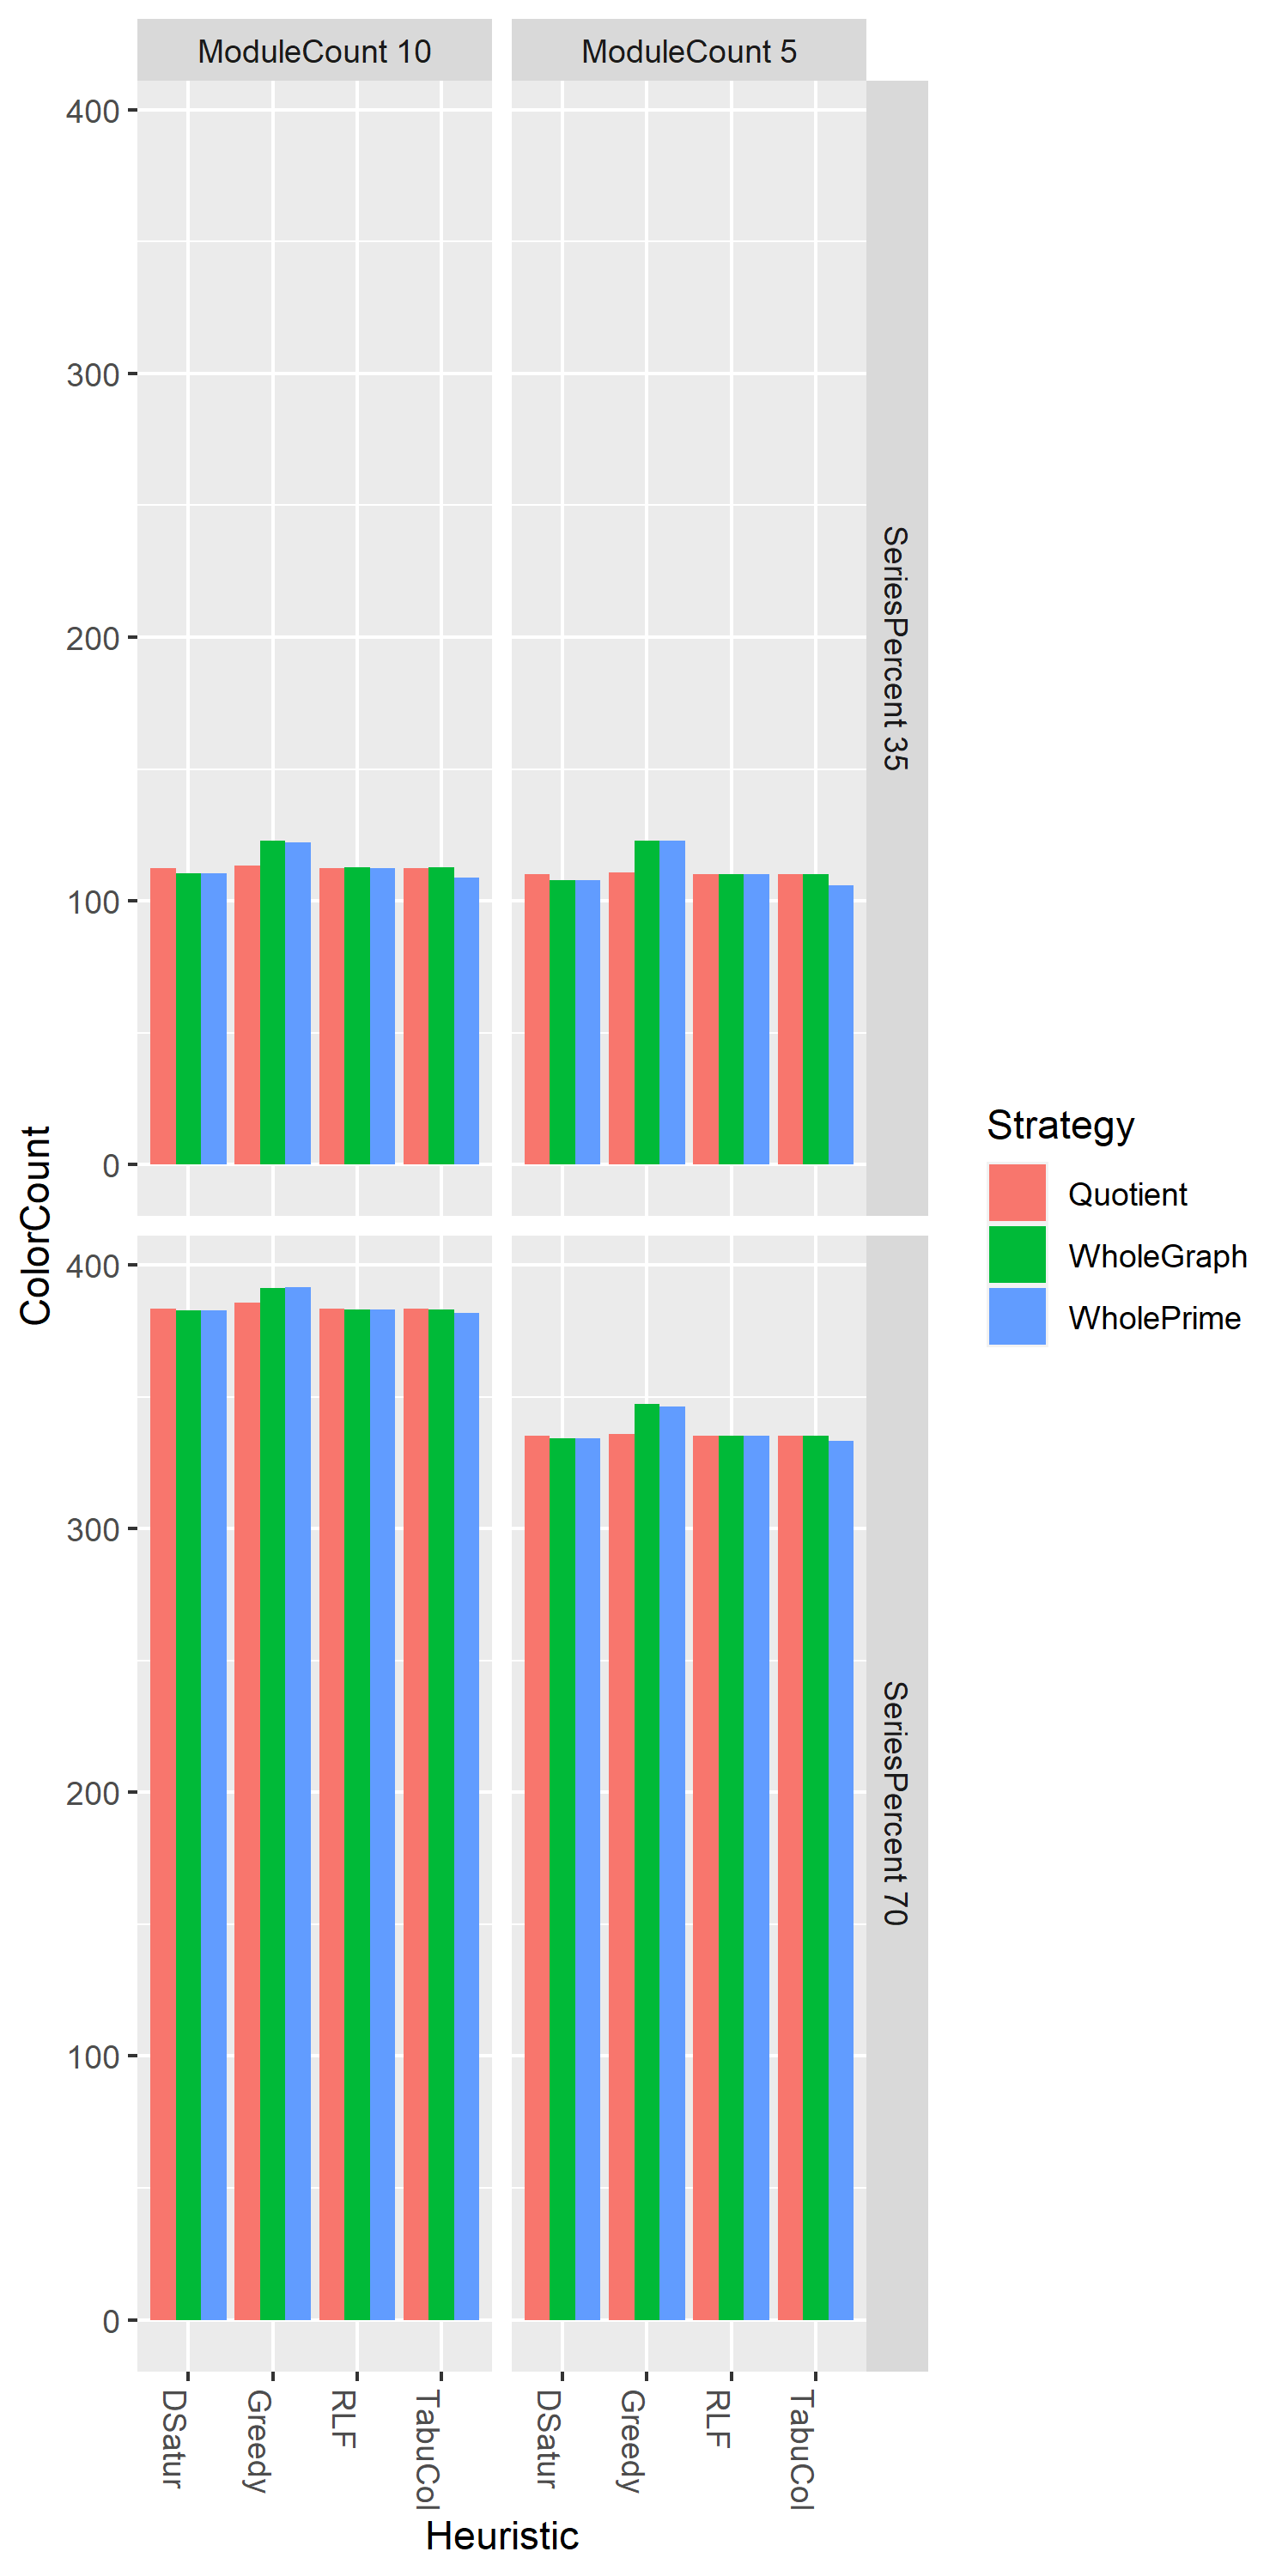
\includegraphics[width=\columnwidth]{Tables/1000.png}
      \caption{Coloring results}
      \label{fig:1000c}
    \end{subfigure}%
    \begin{subfigure}{.4\paperwidth}
        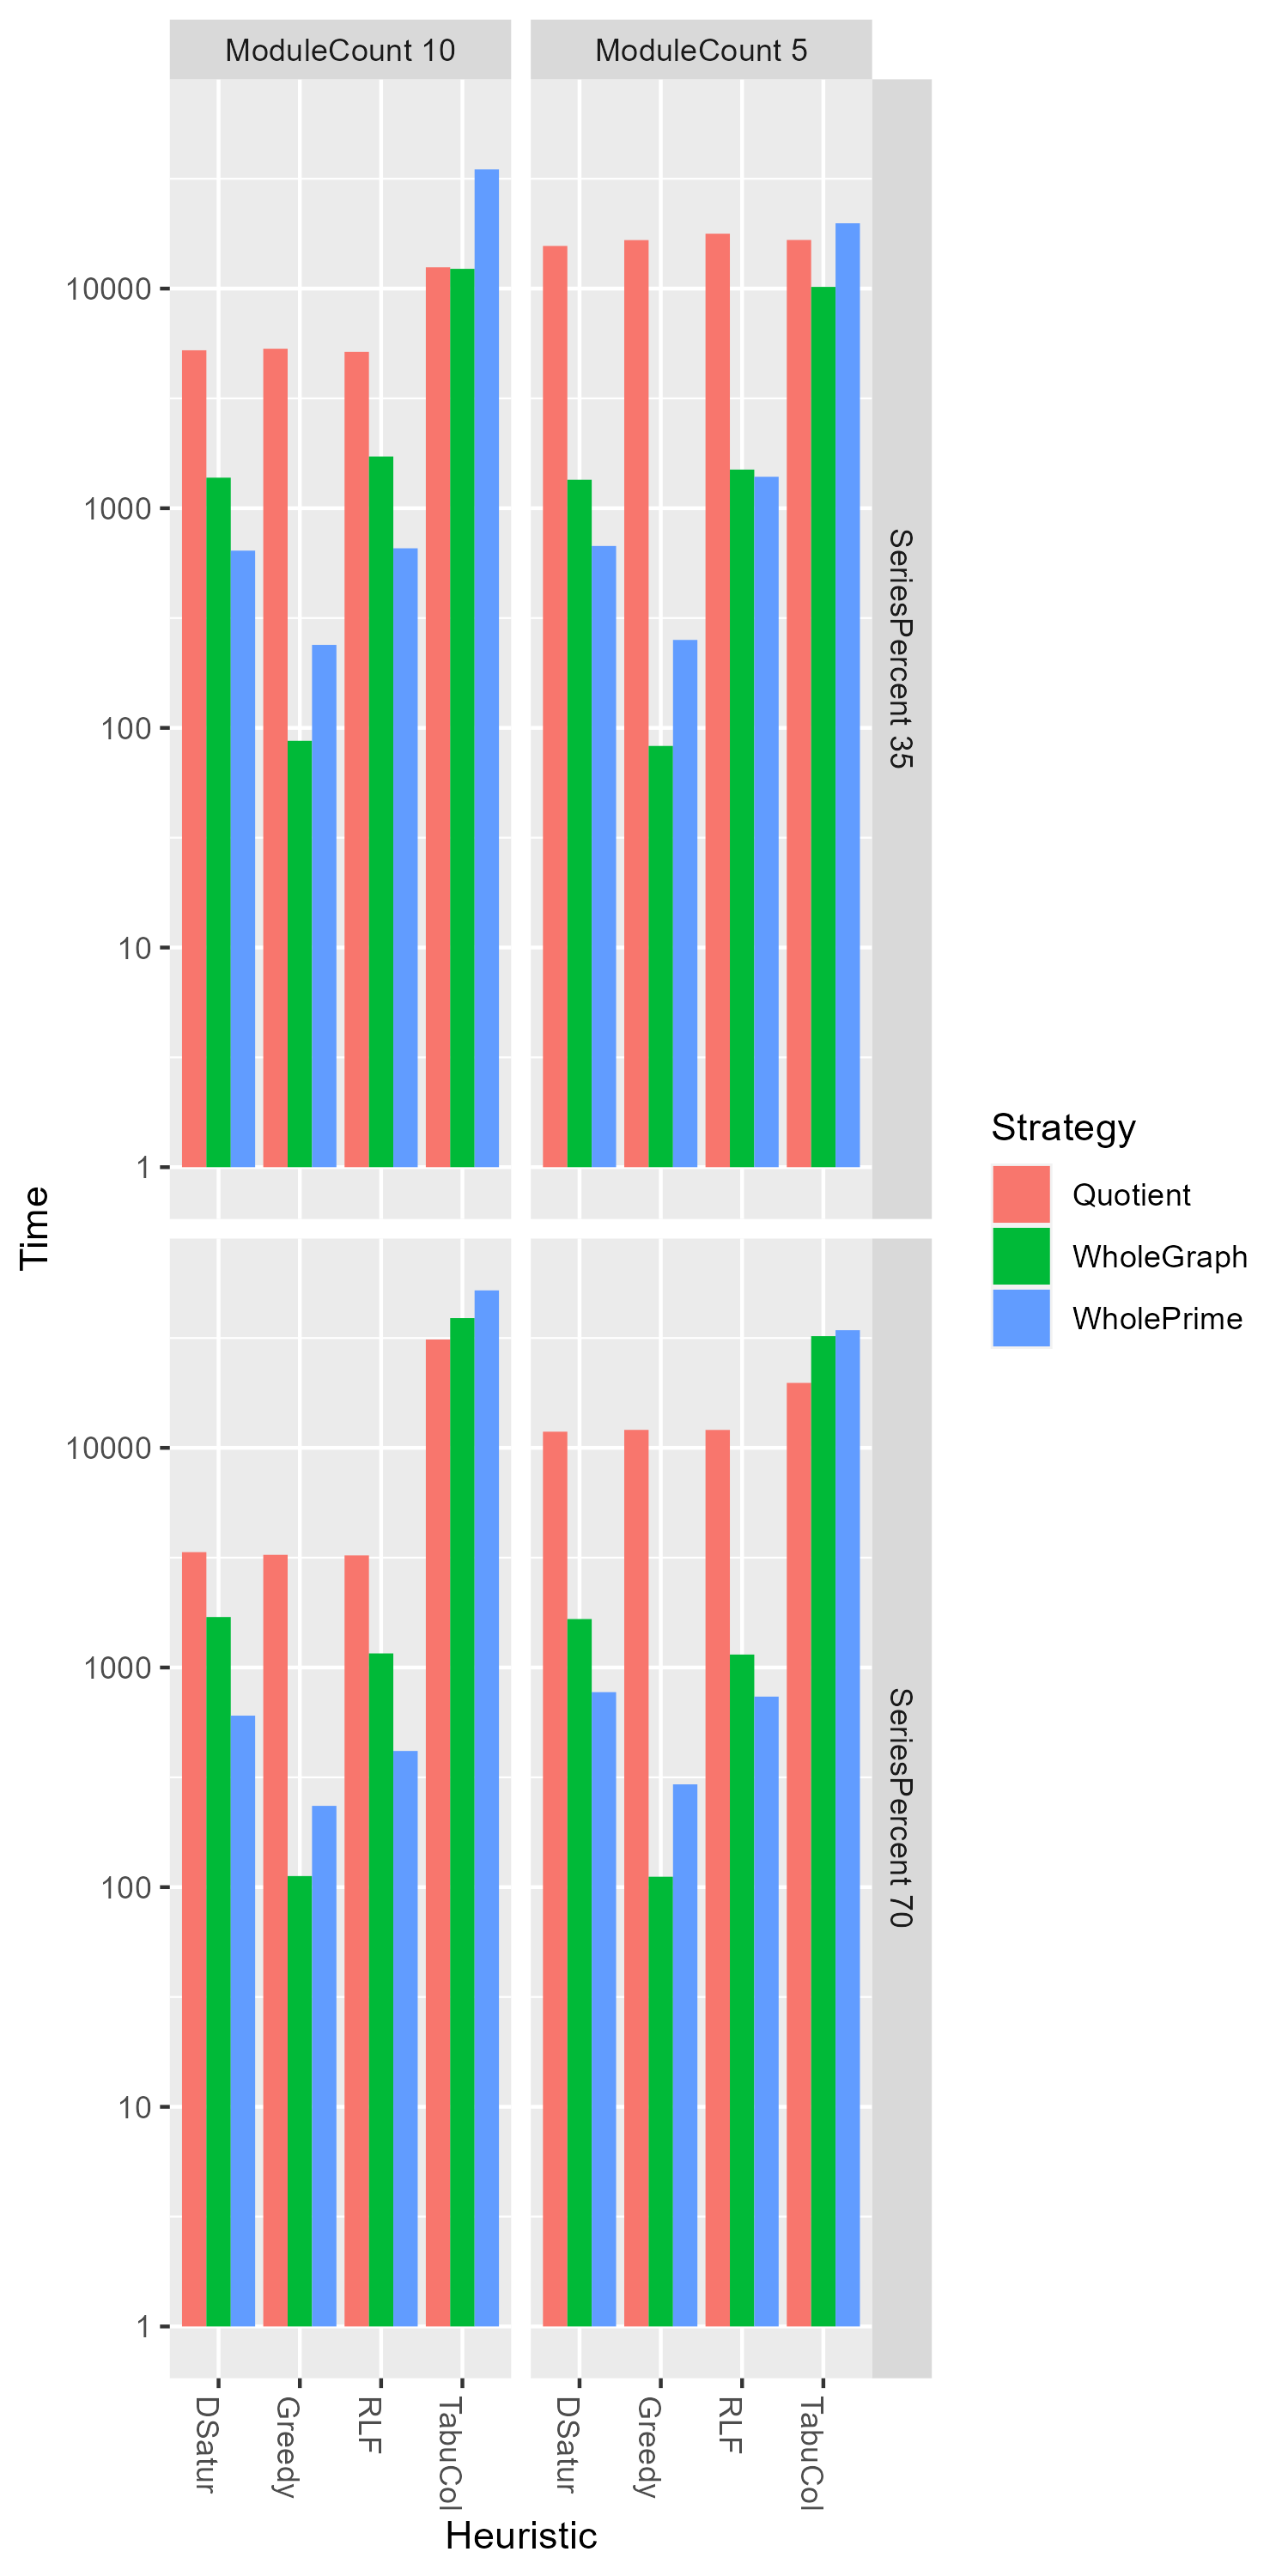
\includegraphics[width=\columnwidth]{Tables/1000Time.png}
      \caption{Runtime}
      \label{fig:1000t}
    \end{subfigure}
\caption{Result for generated graphs with 1000 vertices. \facfigdesc }
\label{fig:1000}
\end{figure}

\begin{figure}[p]
\centerfloat
    \begin{subfigure}{.4\paperwidth}
        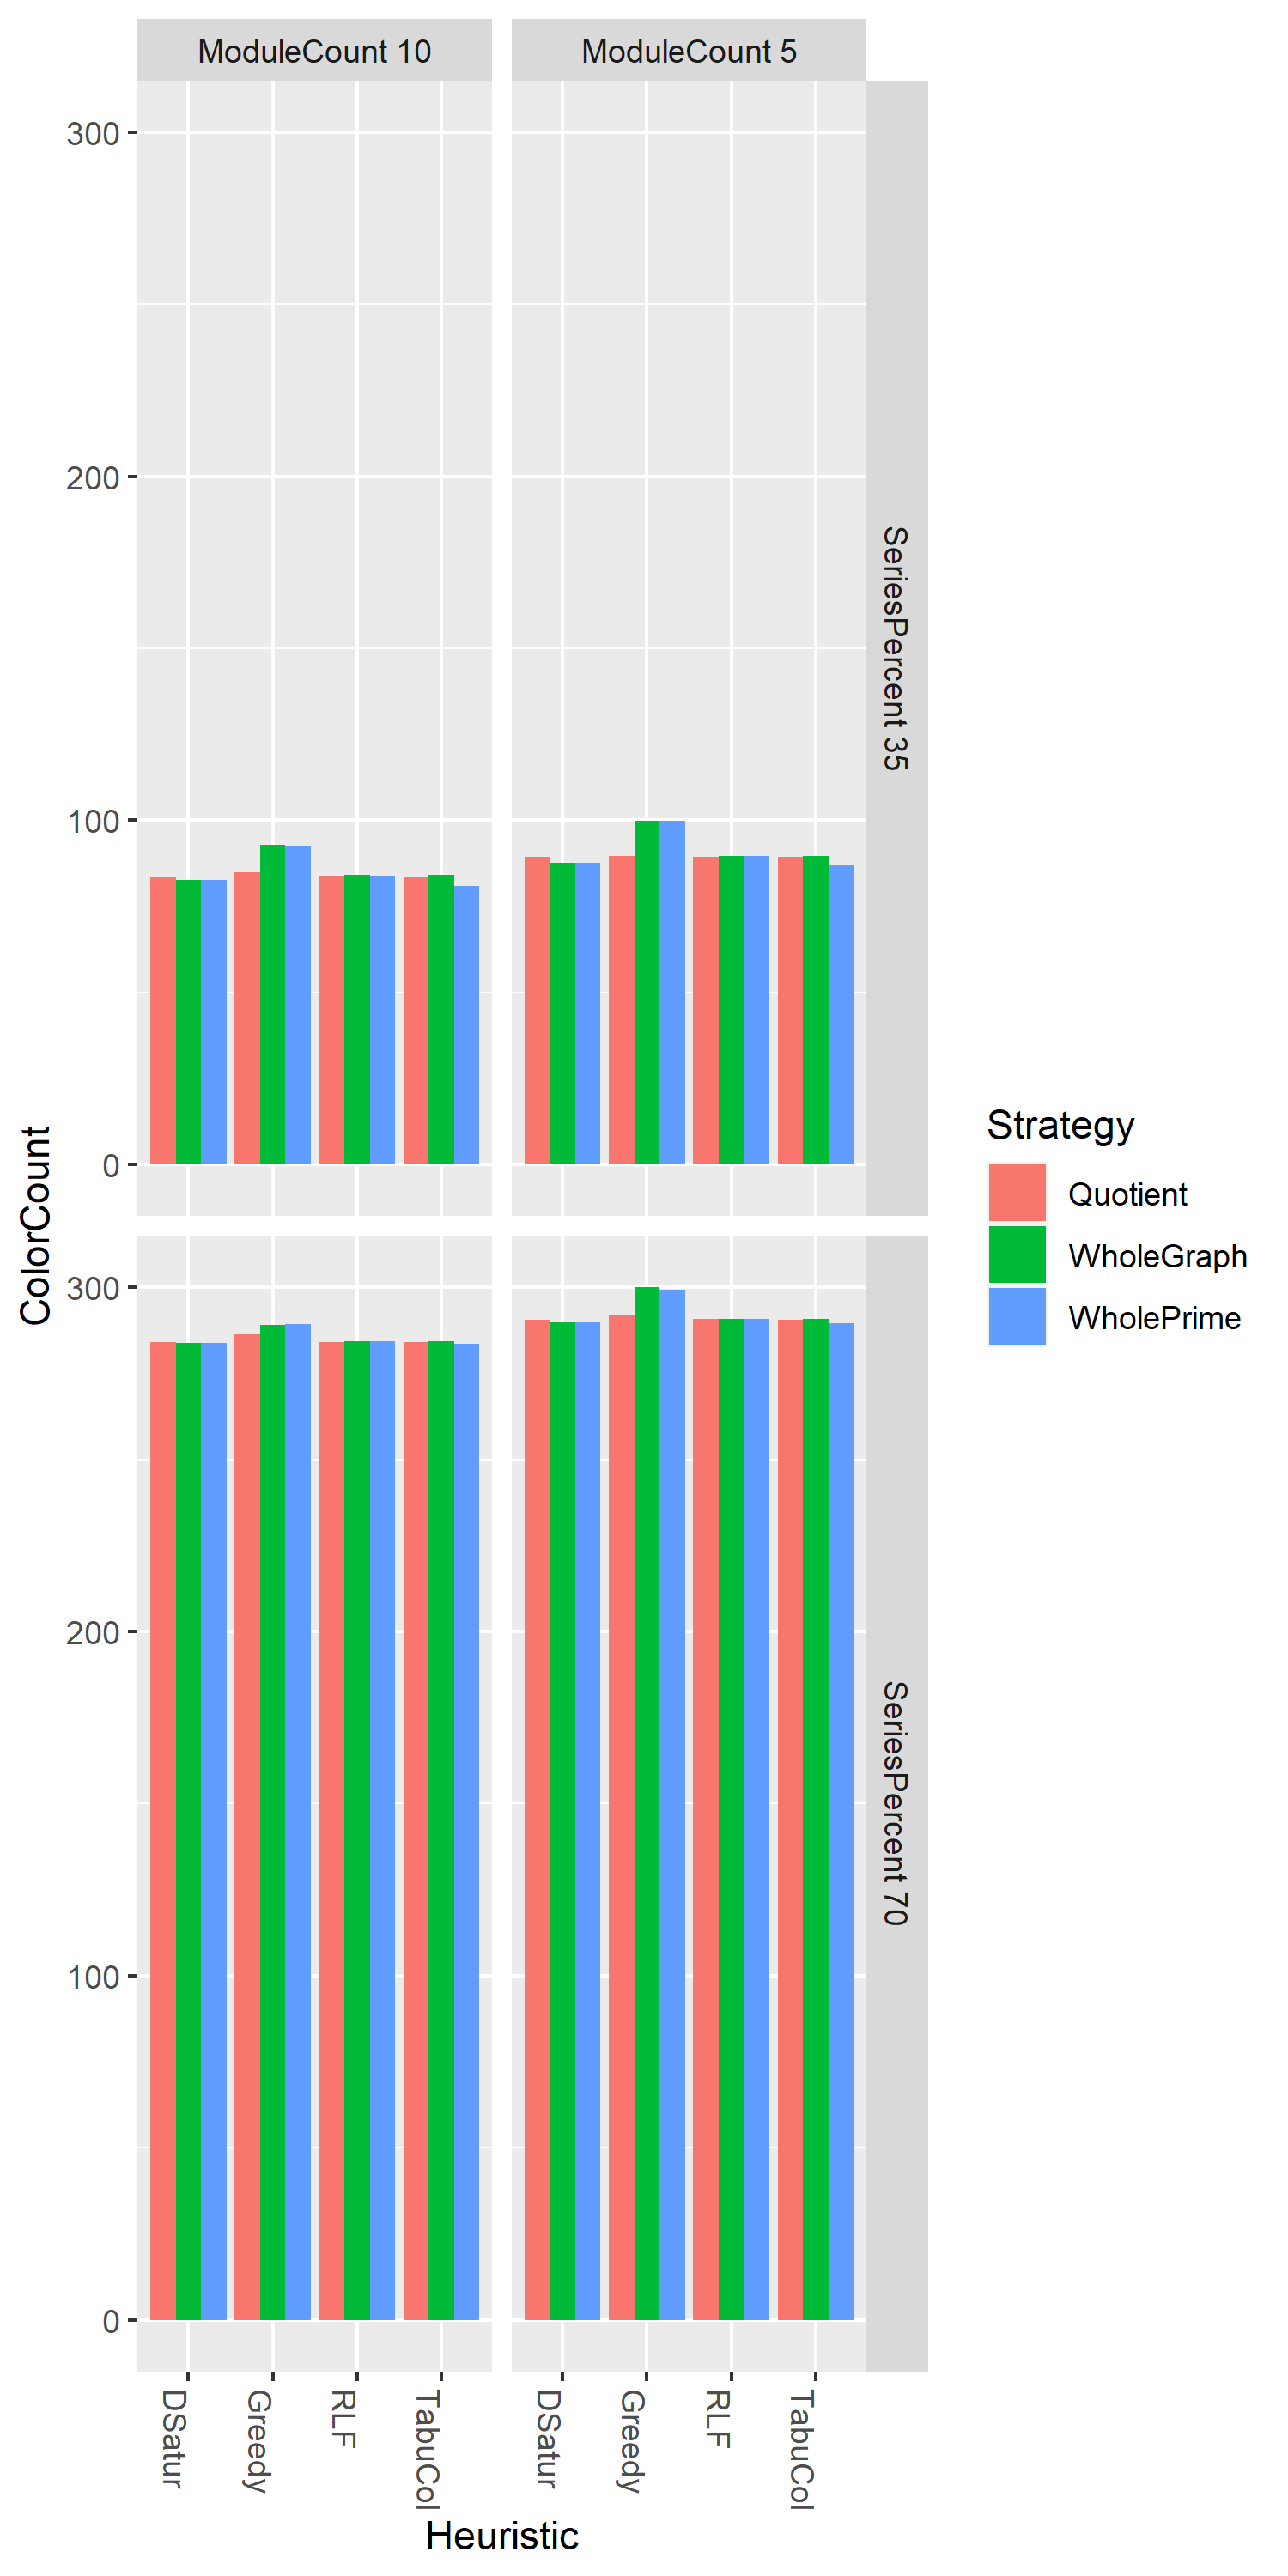
\includegraphics[width=\columnwidth]{Tables/750.png}
      \caption{Coloring results}
      \label{fig:750c}
    \end{subfigure}%
    \begin{subfigure}{.4\paperwidth}
        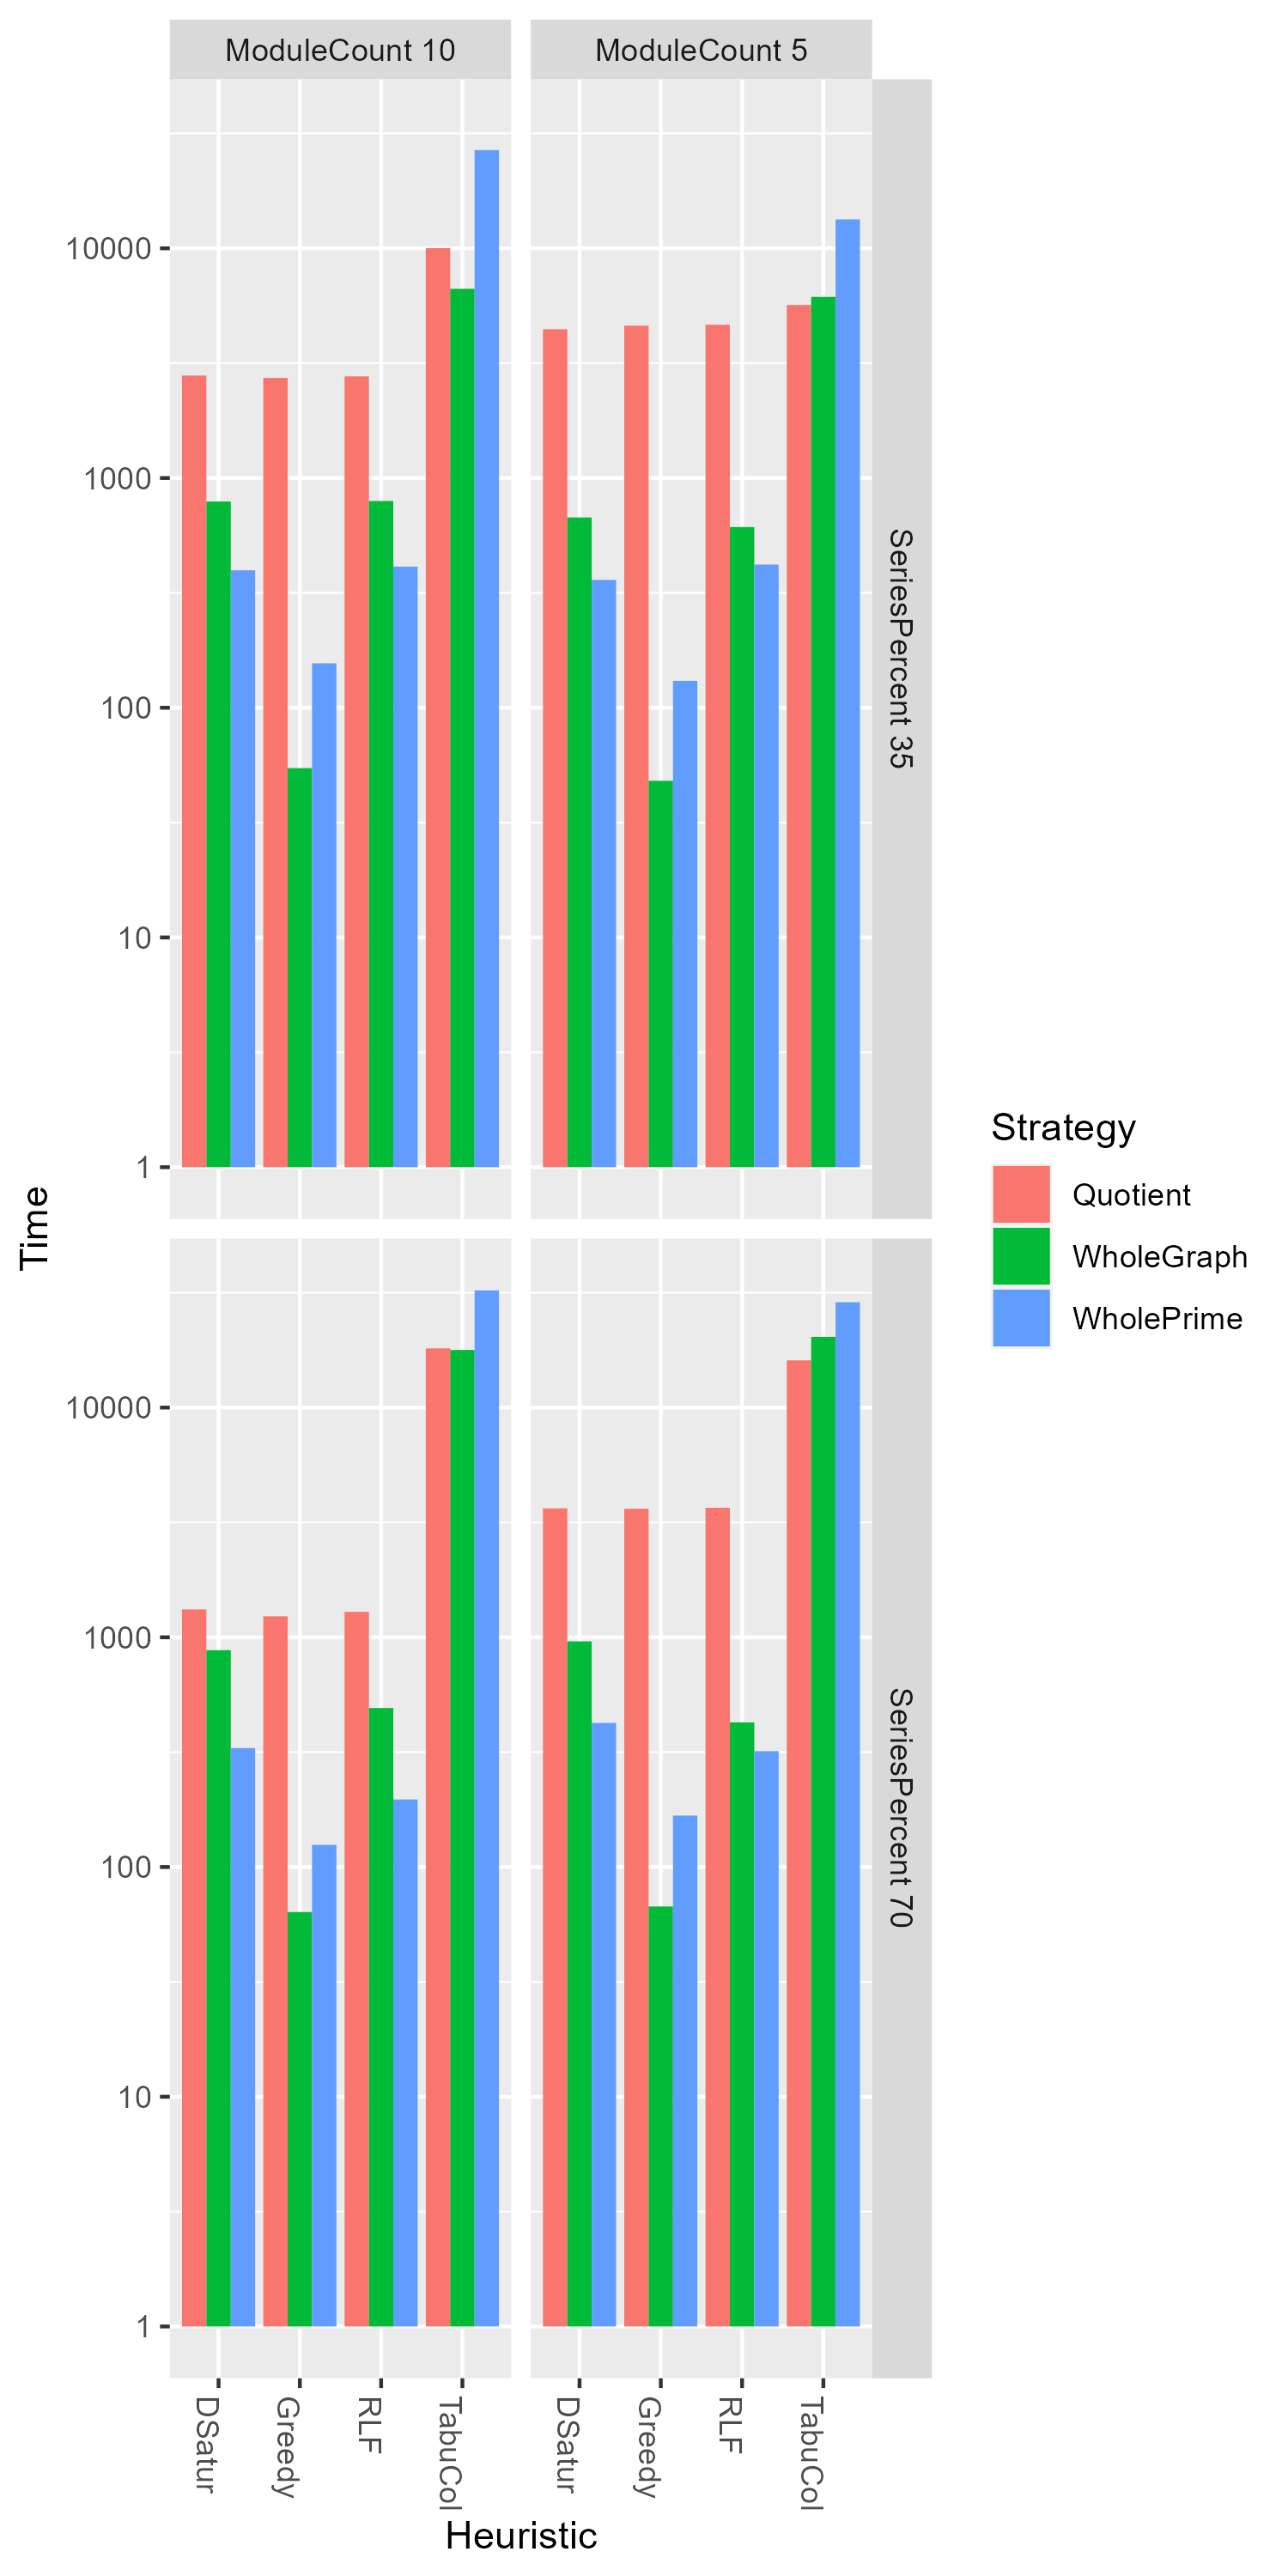
\includegraphics[width=\columnwidth]{Tables/750Time.png}
      \caption{Runtime}
      \label{fig:750t}
    \end{subfigure}
\caption{Result for generated graphs with 750 vertices. \facfigdesc }
\label{fig:750}
\end{figure}

\begin{figure}[p]
\centerfloat
    \begin{subfigure}{.4\paperwidth}
        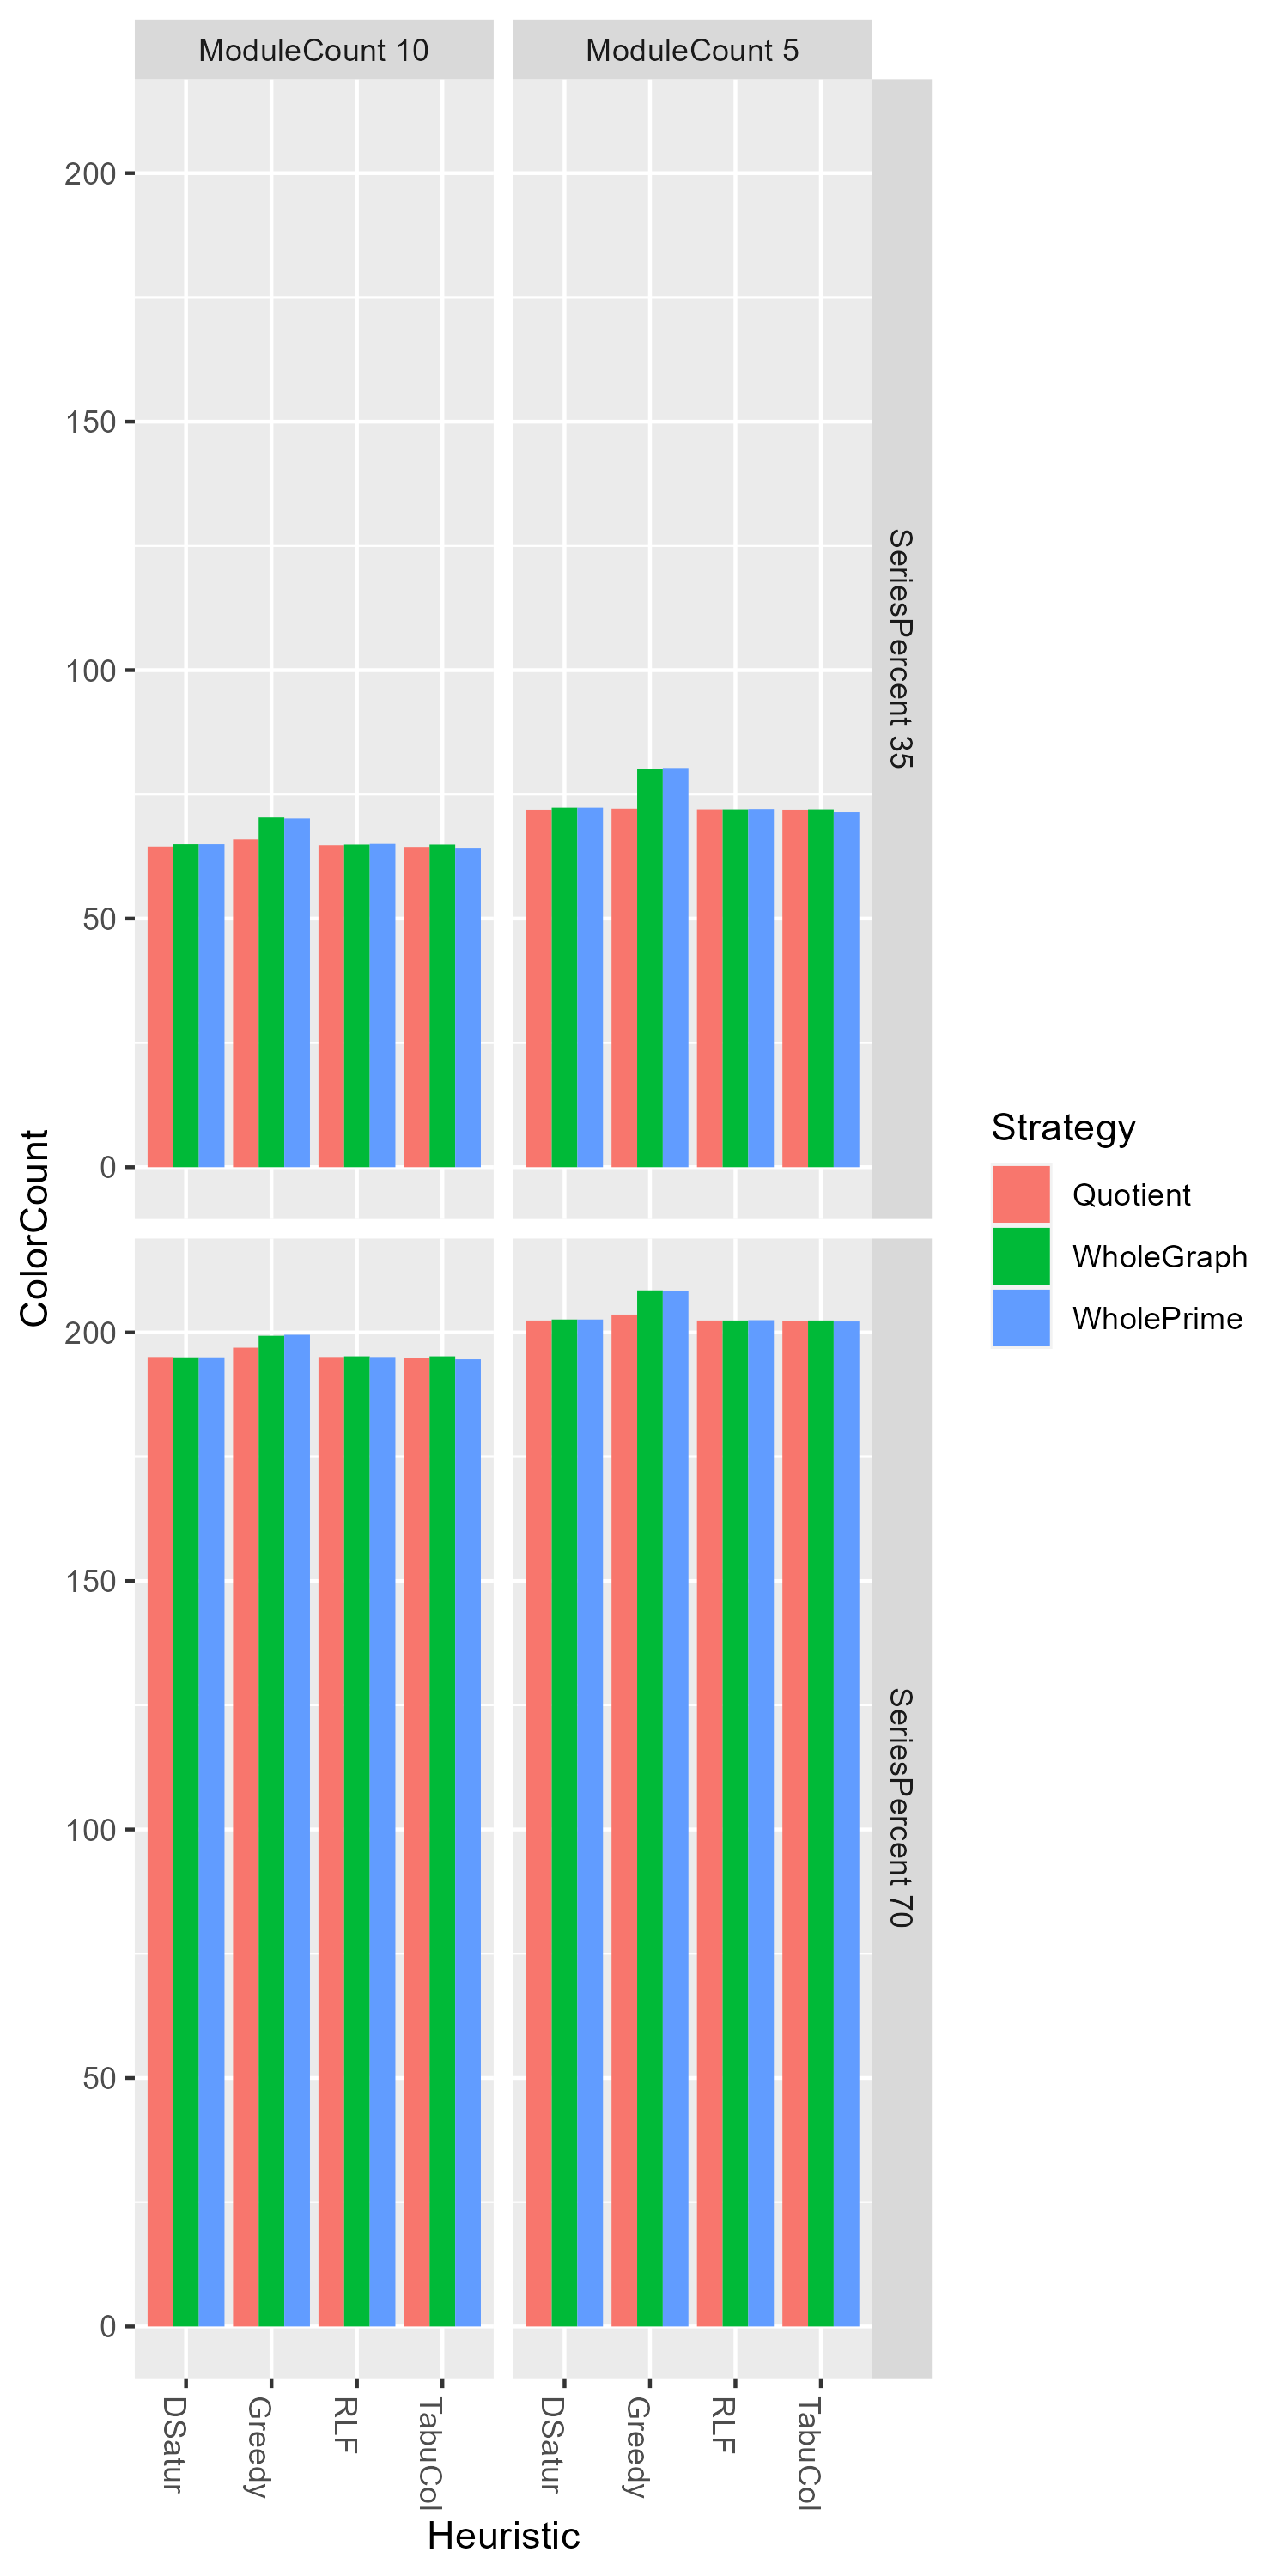
\includegraphics[width=\columnwidth]{Tables/500.png}
      \caption{Coloring results}
      \label{fig:500c}
    \end{subfigure}%
    \begin{subfigure}{.4\paperwidth}
        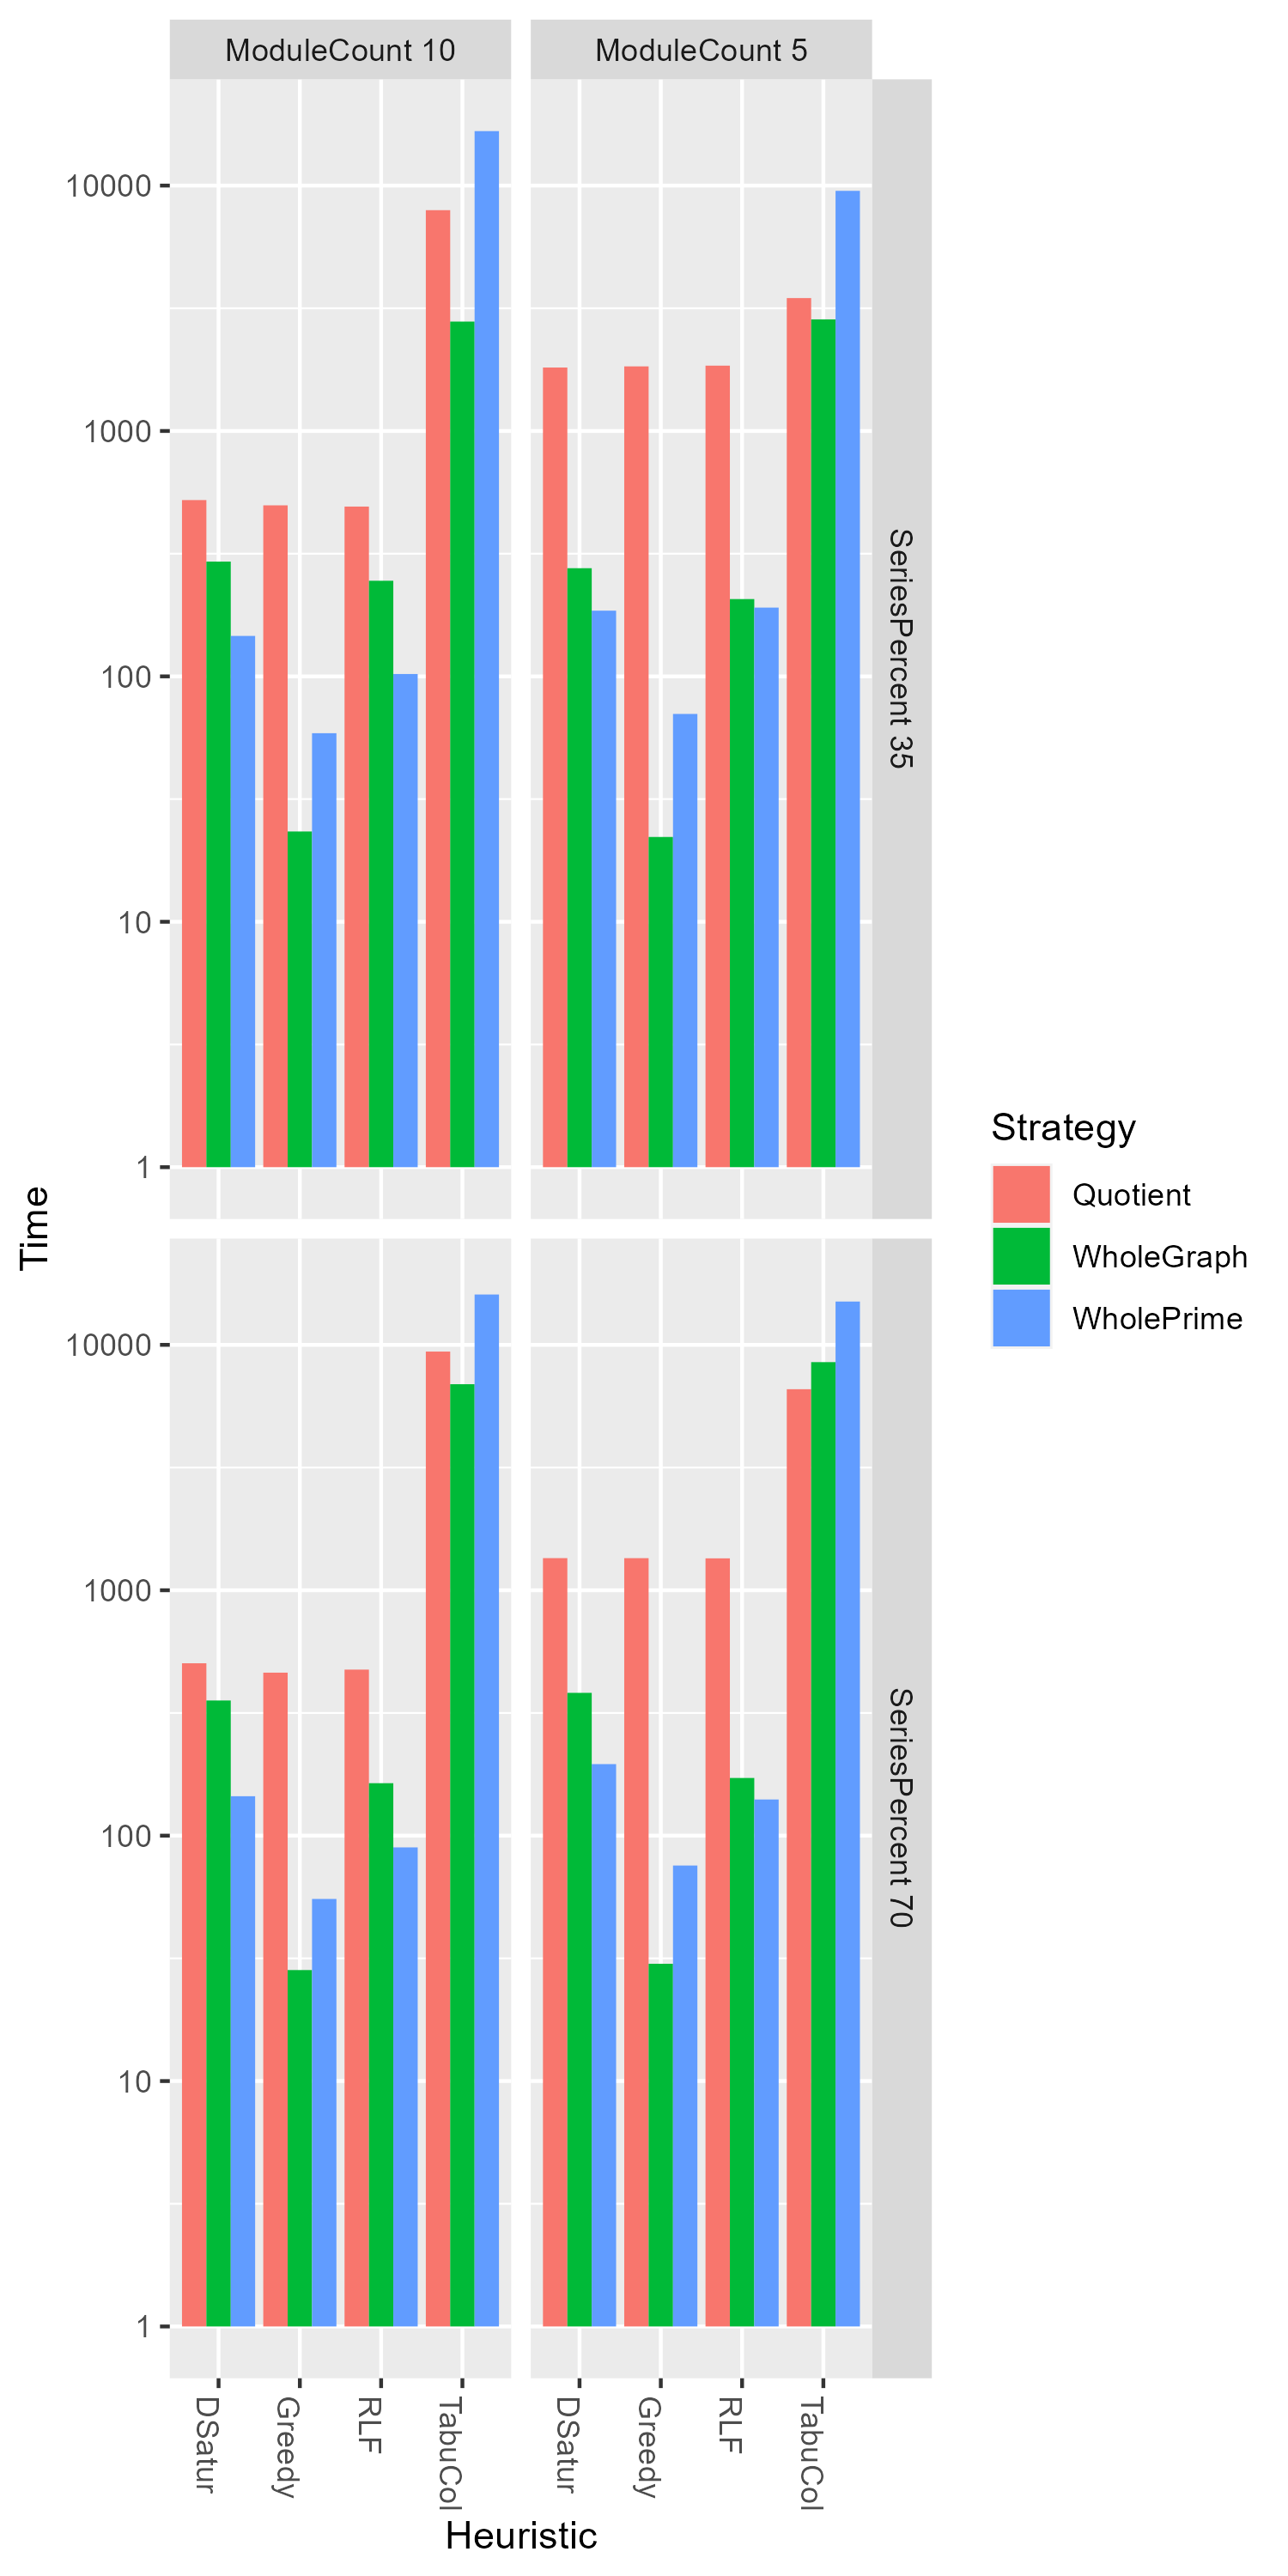
\includegraphics[width=\columnwidth]{Tables/500Time.png}
      \caption{Runtime}
      \label{fig:500t}
    \end{subfigure}
\caption{Result for generated graphs with 500 vertices. \facfigdesc}
\label{fig:500}
\end{figure}


\begin{figure}[p]
\centerfloat
    \begin{subfigure}{.4\paperwidth}
        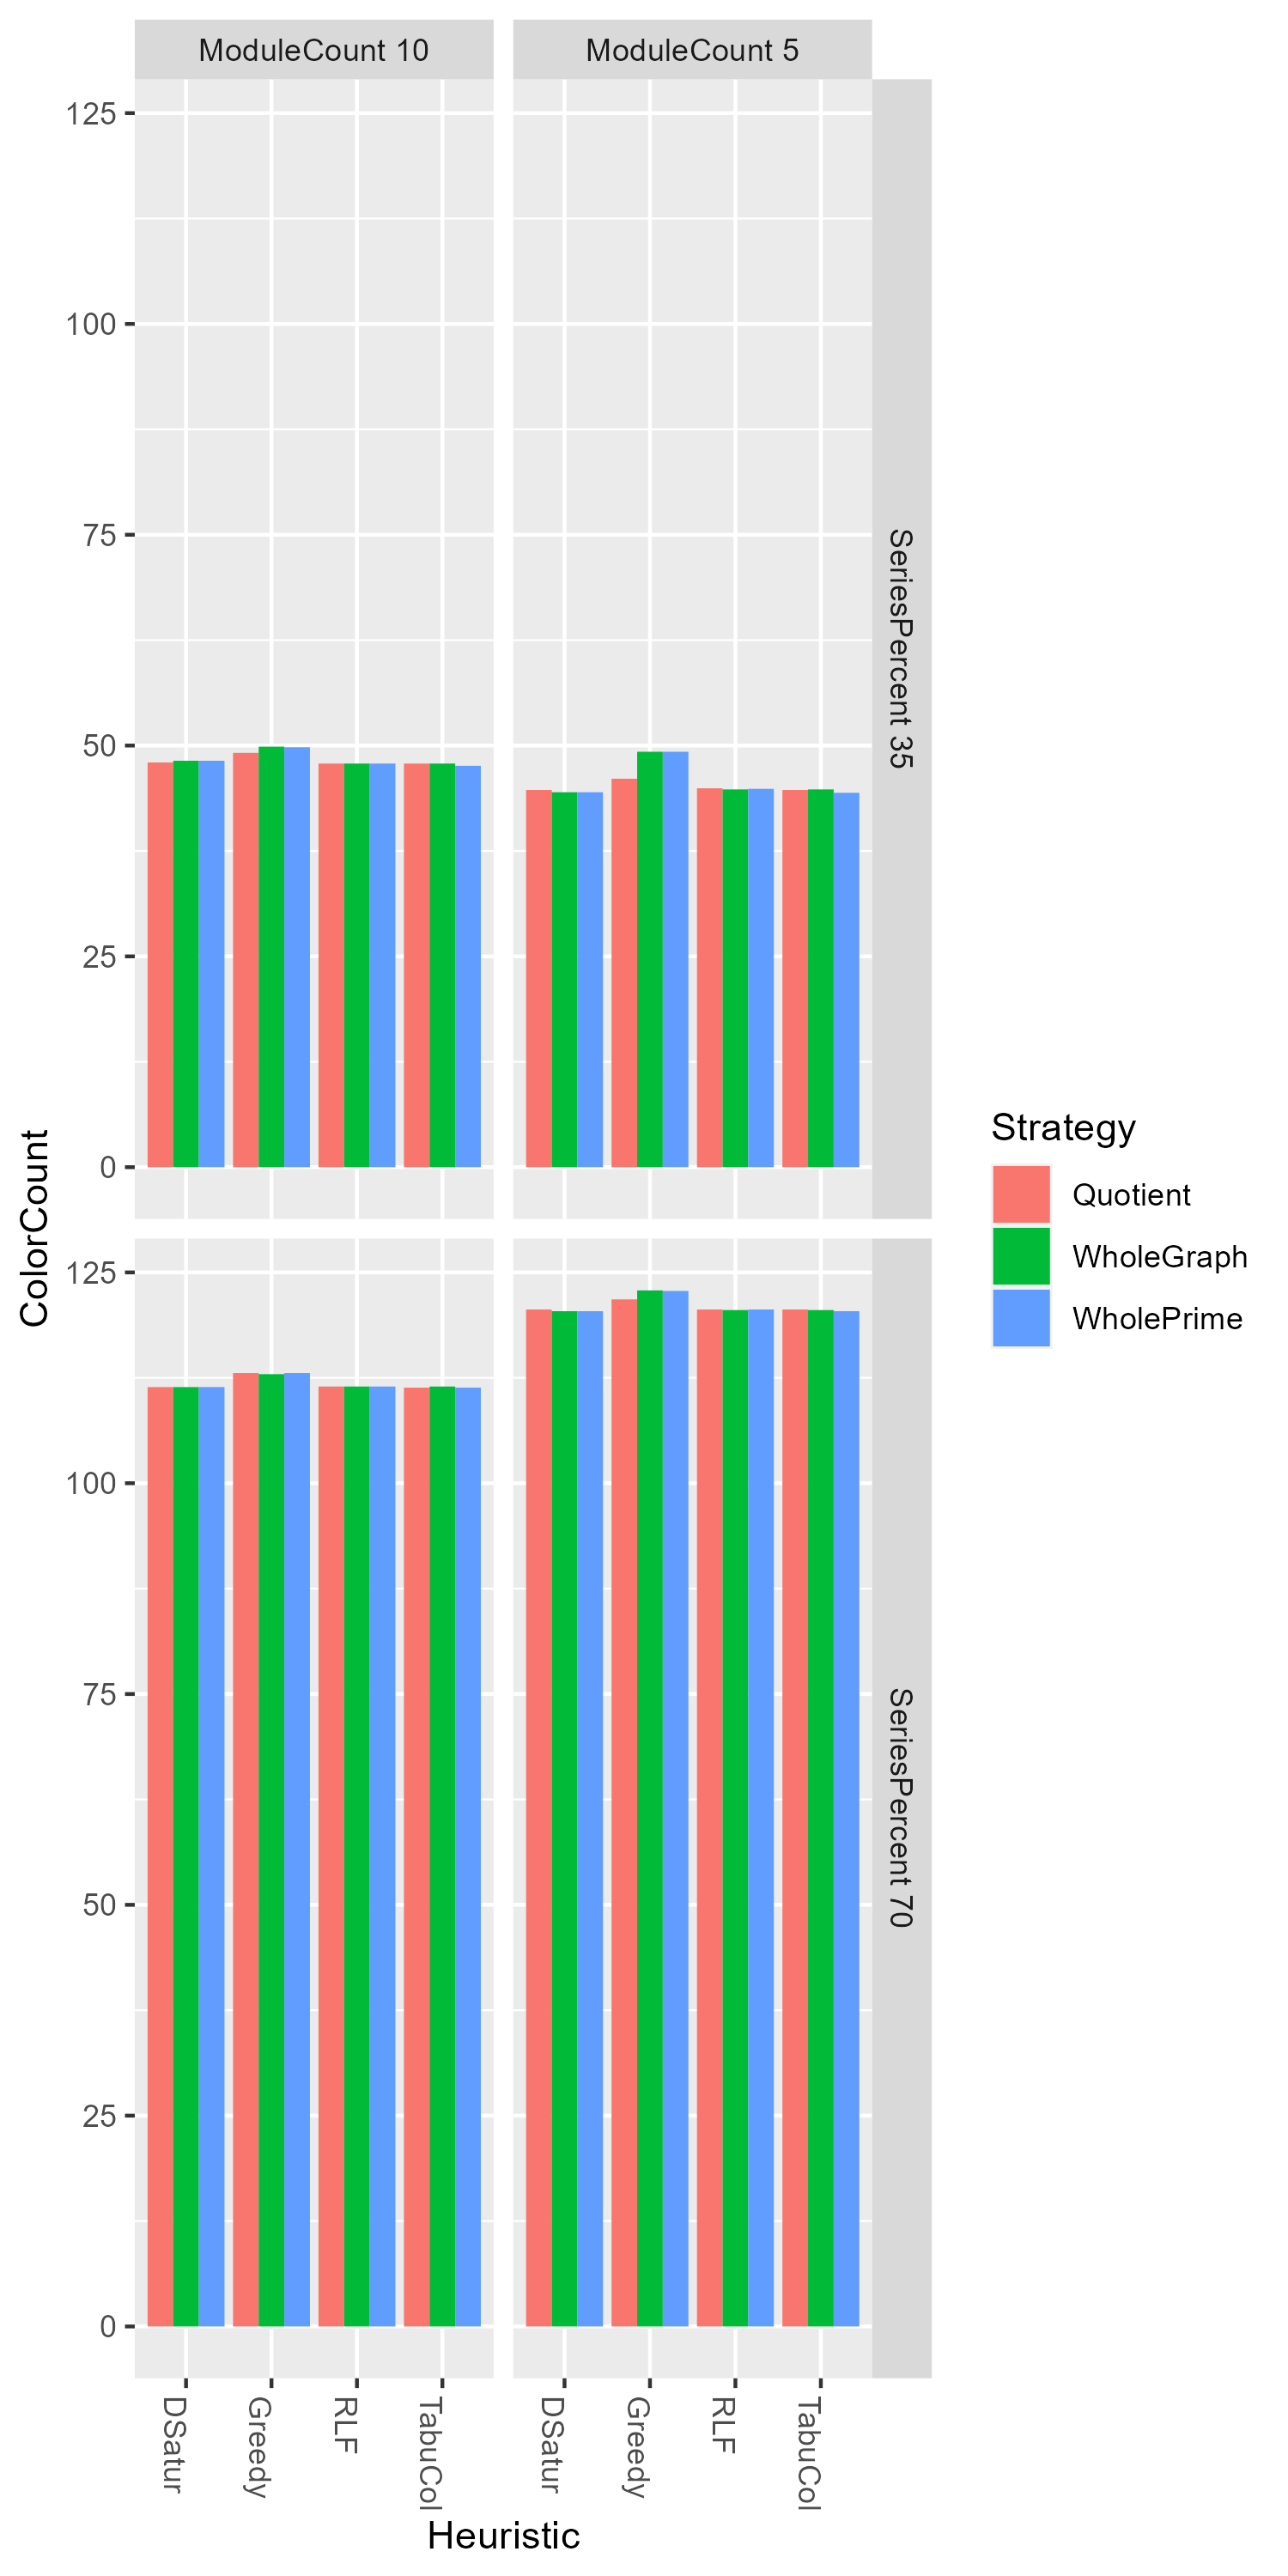
\includegraphics[width=\columnwidth]{Tables/250.png}
      \caption{Coloring results}
      \label{fig:250c}
    \end{subfigure}%
    \begin{subfigure}{.4\paperwidth}
        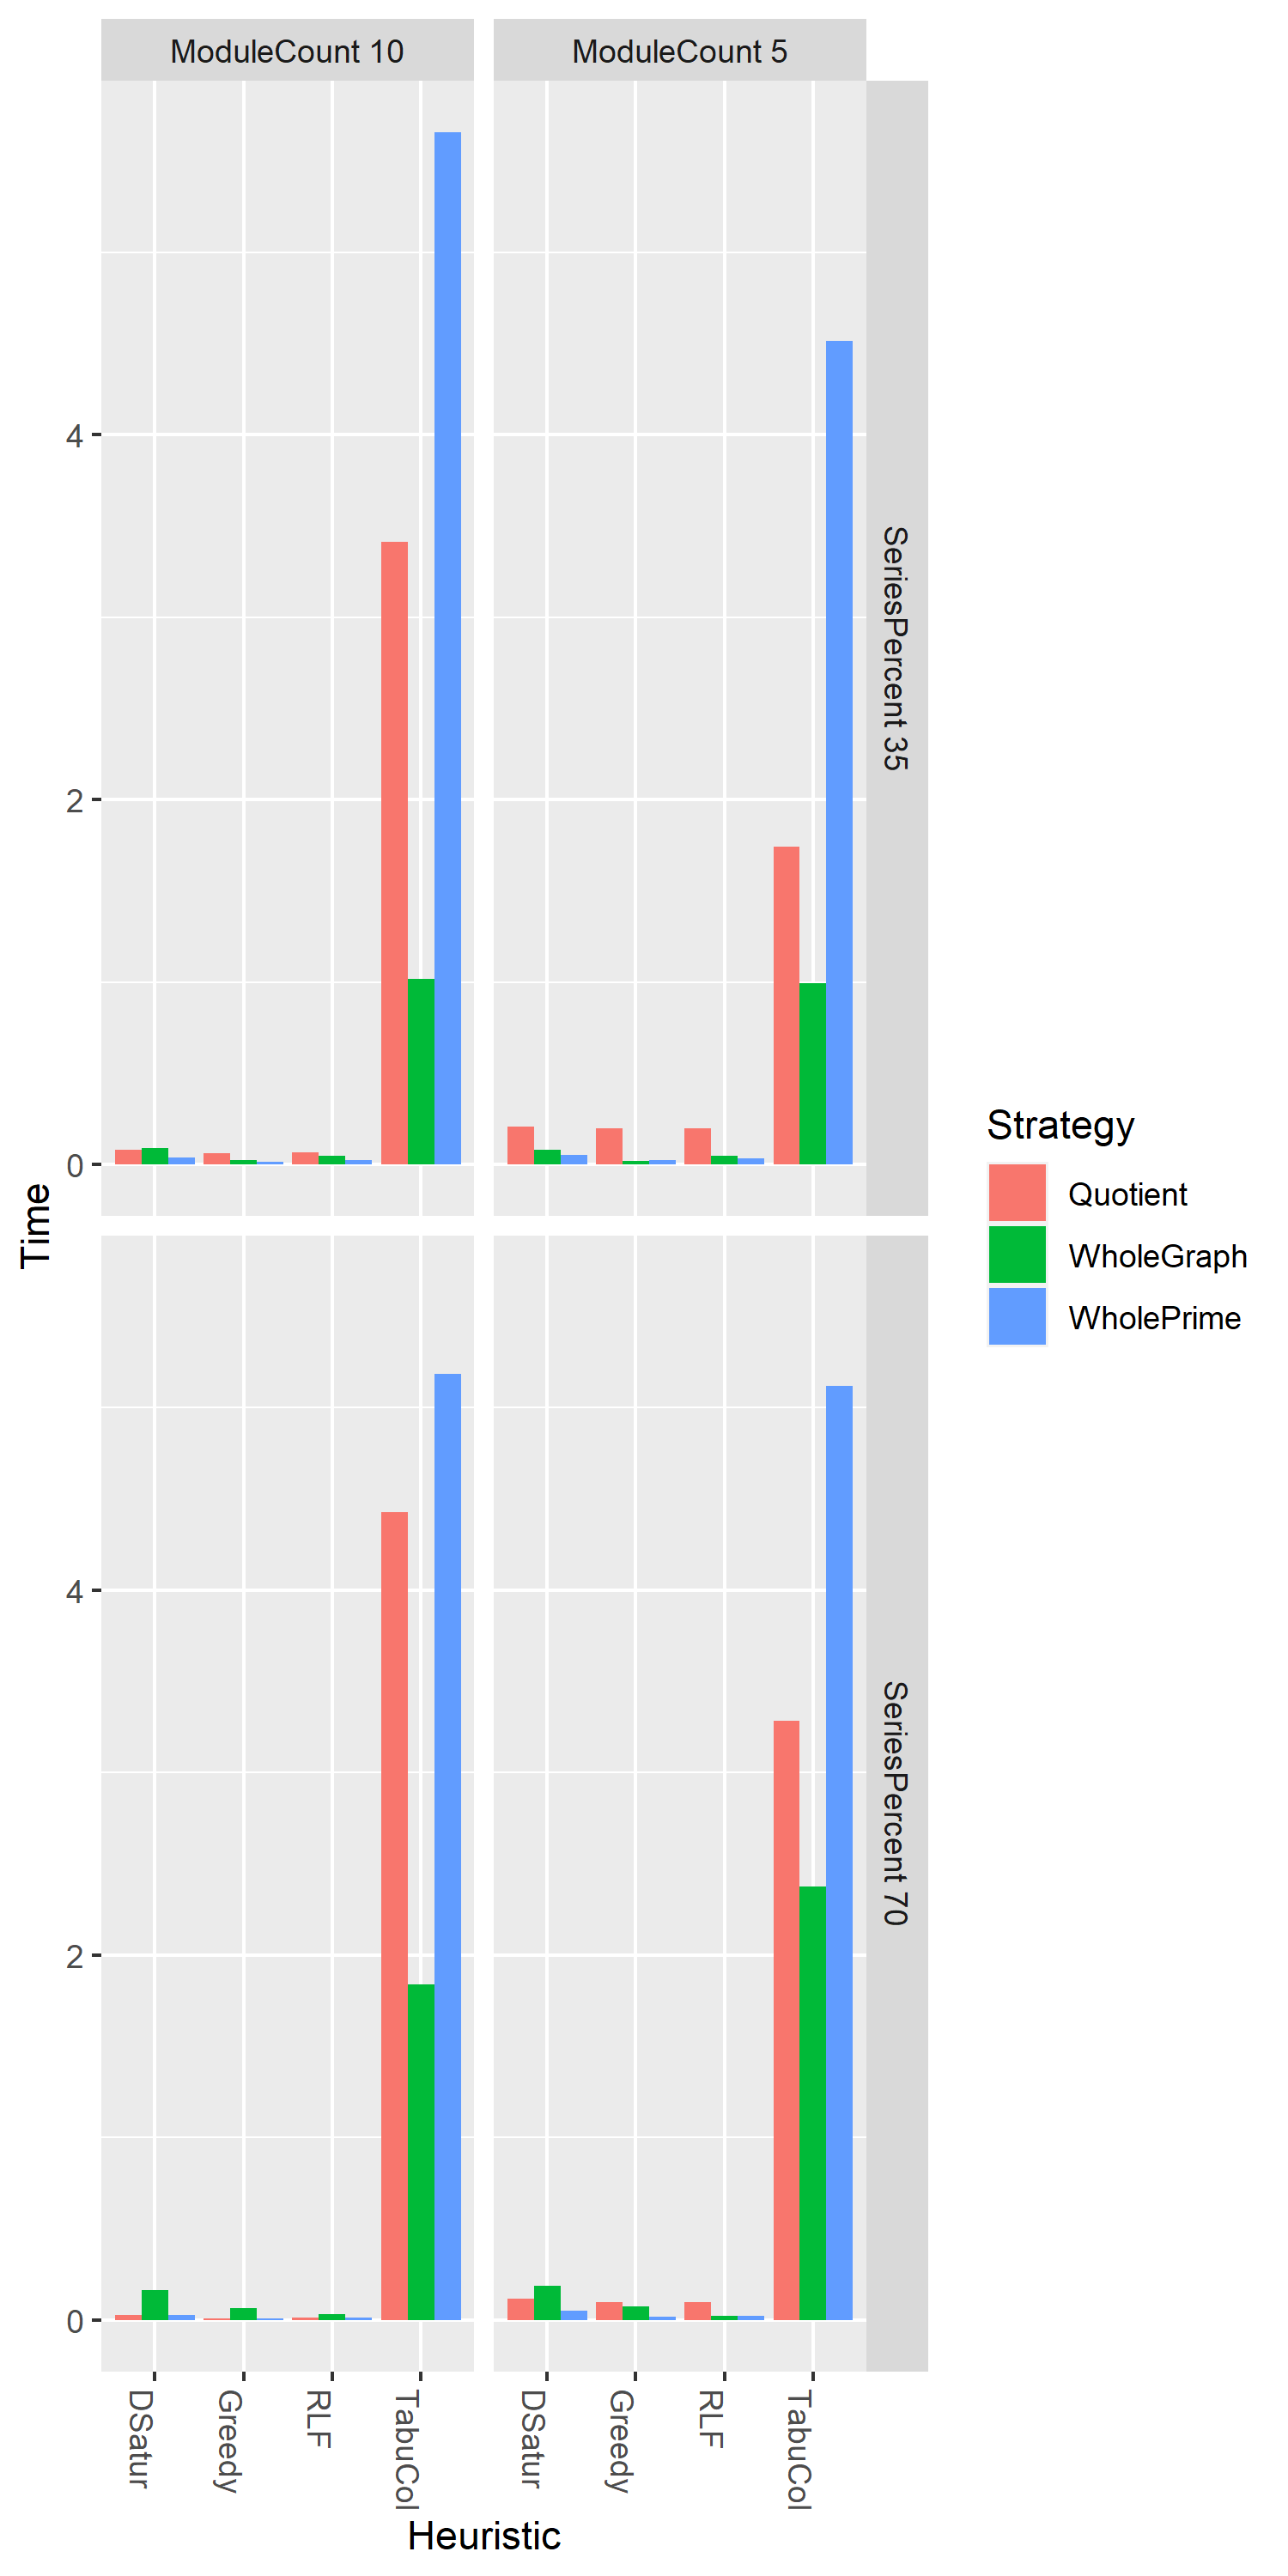
\includegraphics[width=\columnwidth]{Tables/250Time.png}
      \caption{Runtime}
      \label{fig:250t}
    \end{subfigure}
\caption{Result for generated graphs with 250 vertices. \facfigdesc}
\label{fig:250}
\end{figure}



\begin{figure}[p]
\centerfloat
    \begin{subfigure}{.4\paperwidth}
        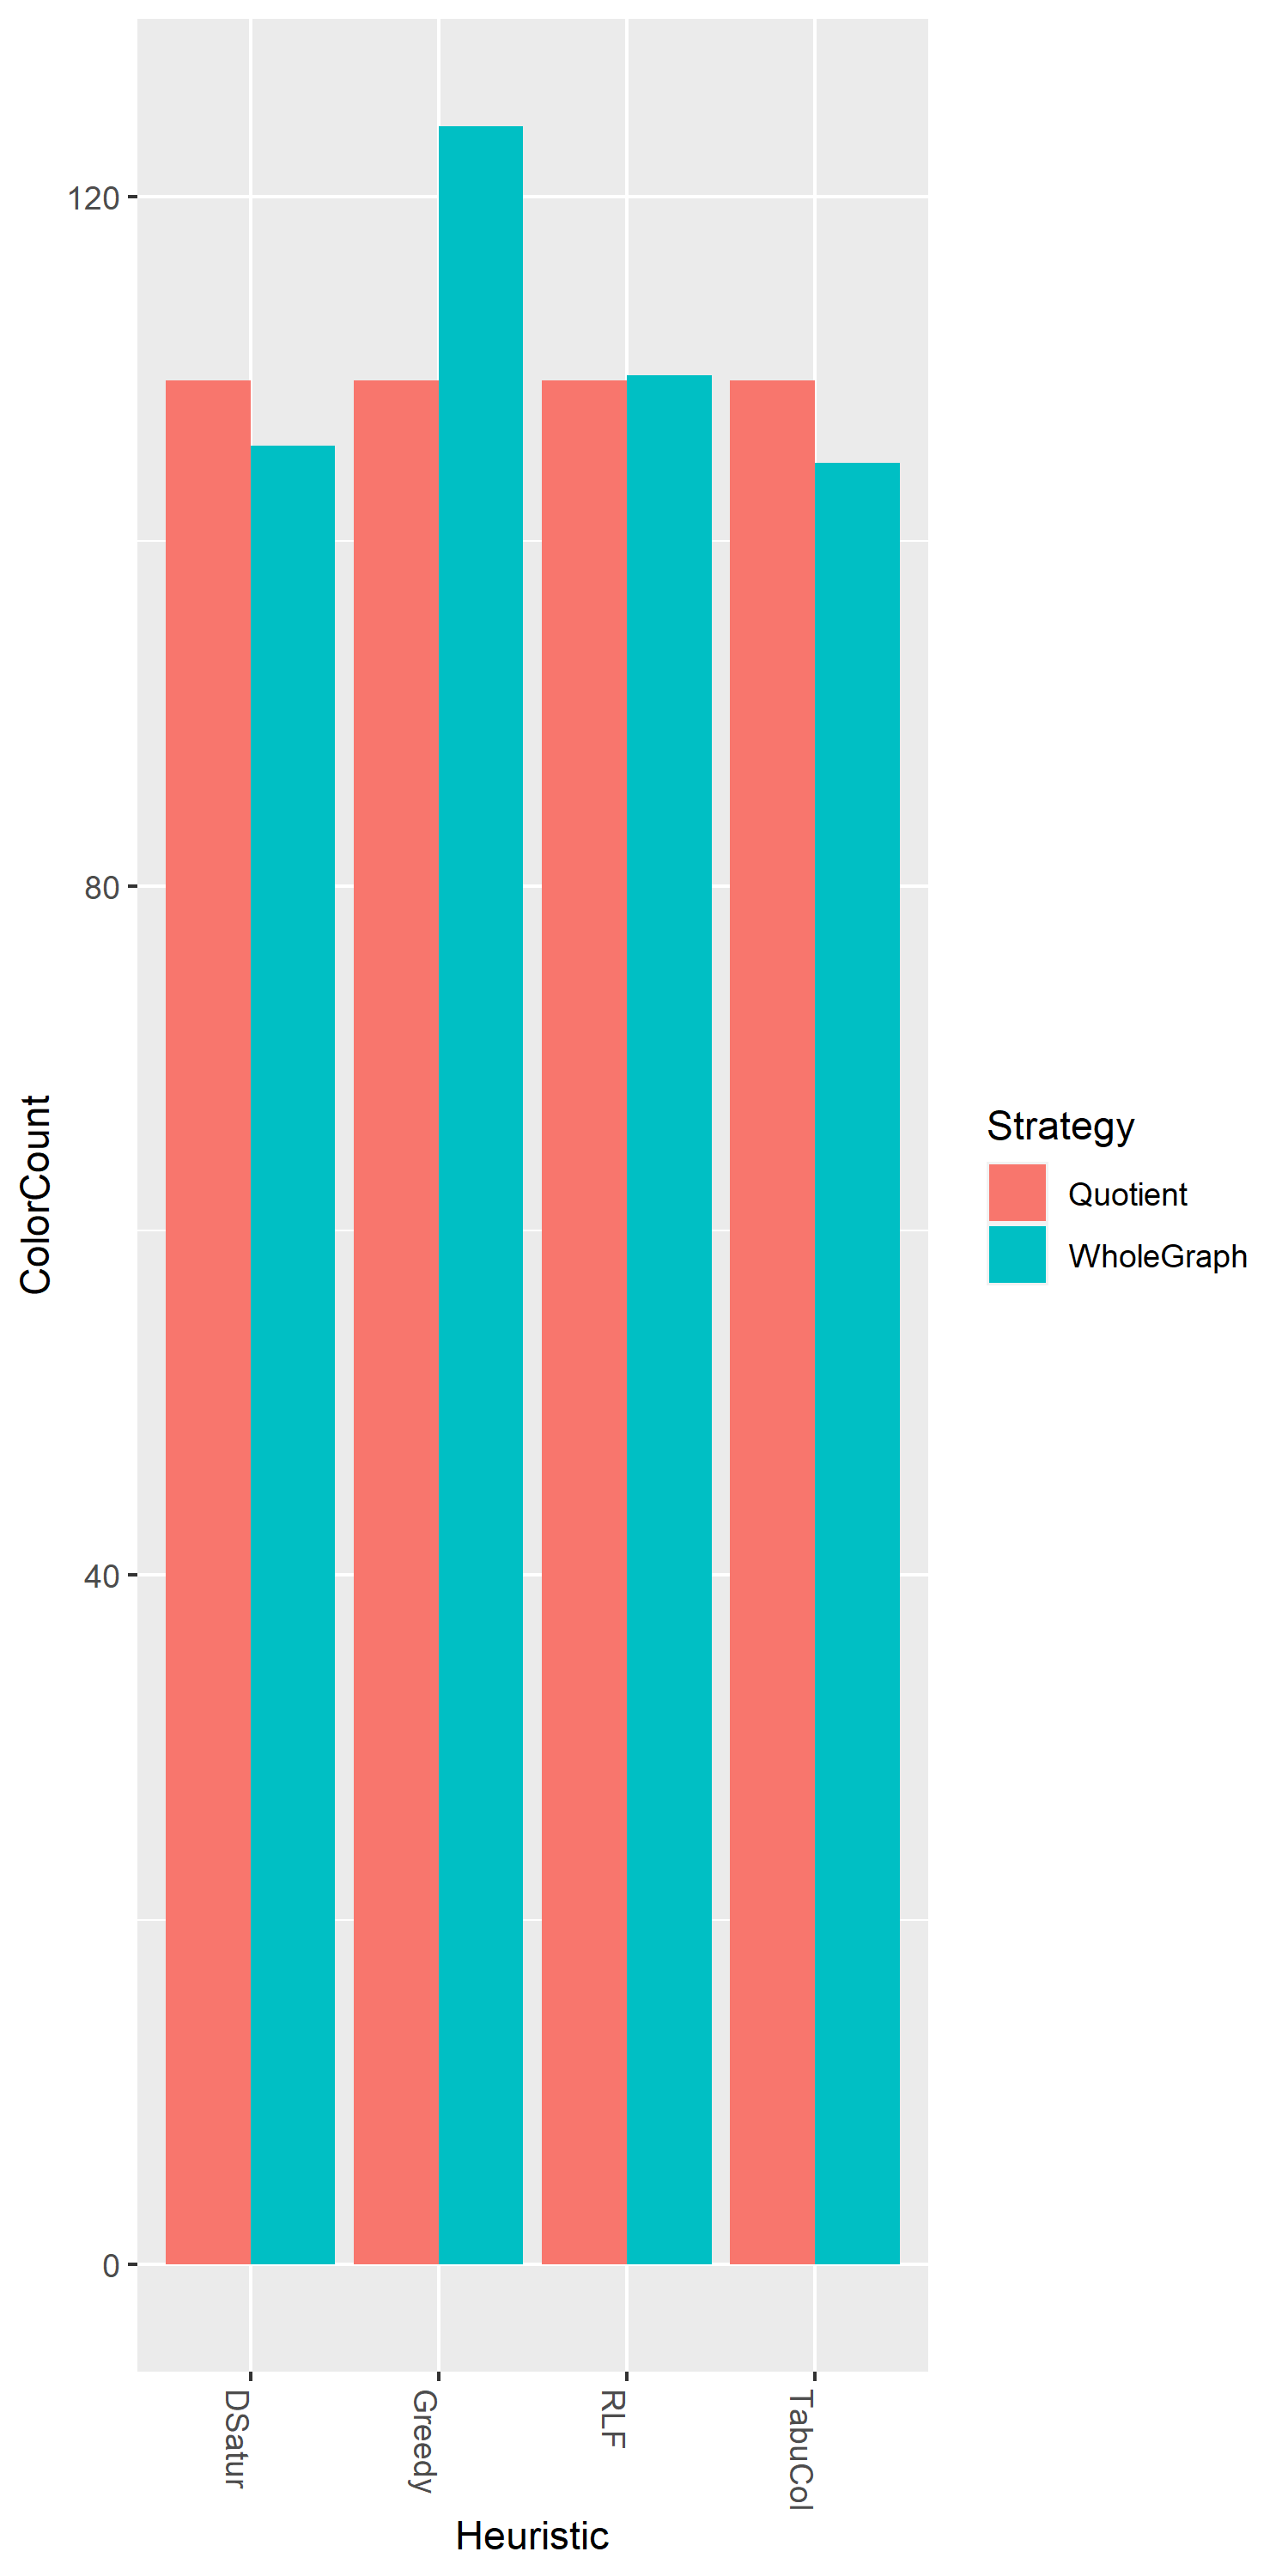
\includegraphics[width=\columnwidth]{Tables/DIMACS.png}
      \caption{Coloring results}
      \label{fig:dimacsc}
    \end{subfigure}%
    \begin{subfigure}{.4\paperwidth}
        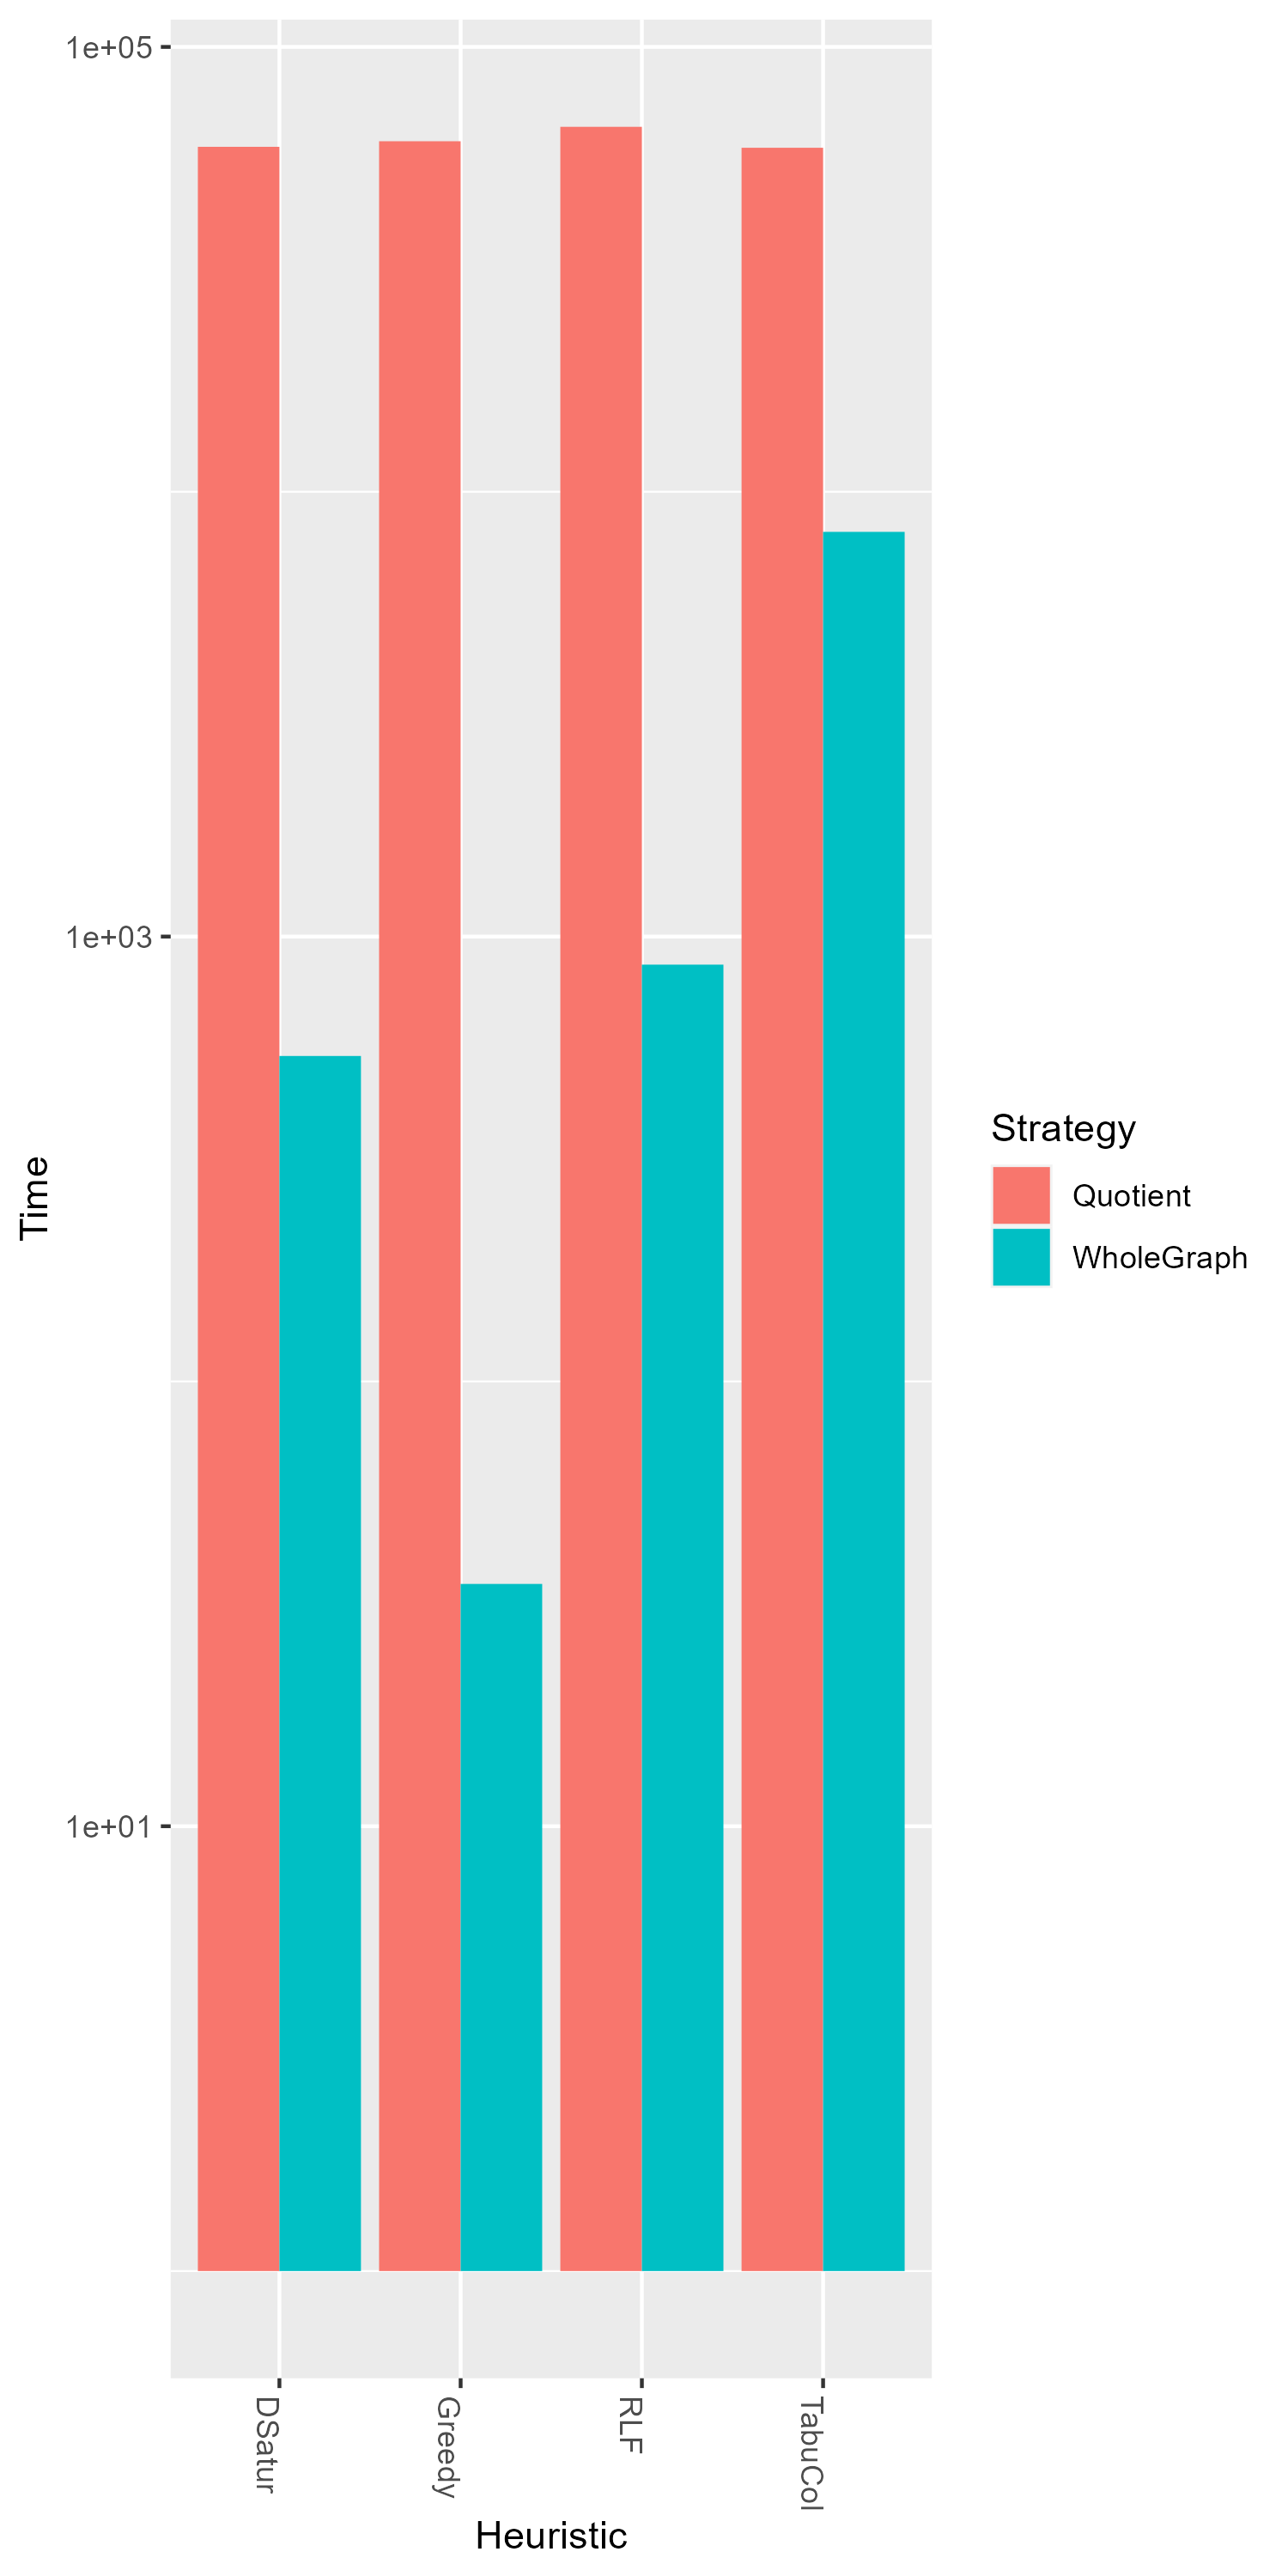
\includegraphics[width=\columnwidth]{Tables/DIMACSTime.png}
      \caption{Runtime}
      \label{fig:dimacst}
    \end{subfigure}
\caption{Result for the DIMACS graphs. \figdesc}
\label{fig:dimacs}
\end{figure}

\begin{figure}[p]
\centerfloat
    \begin{subfigure}{.4\paperwidth}
        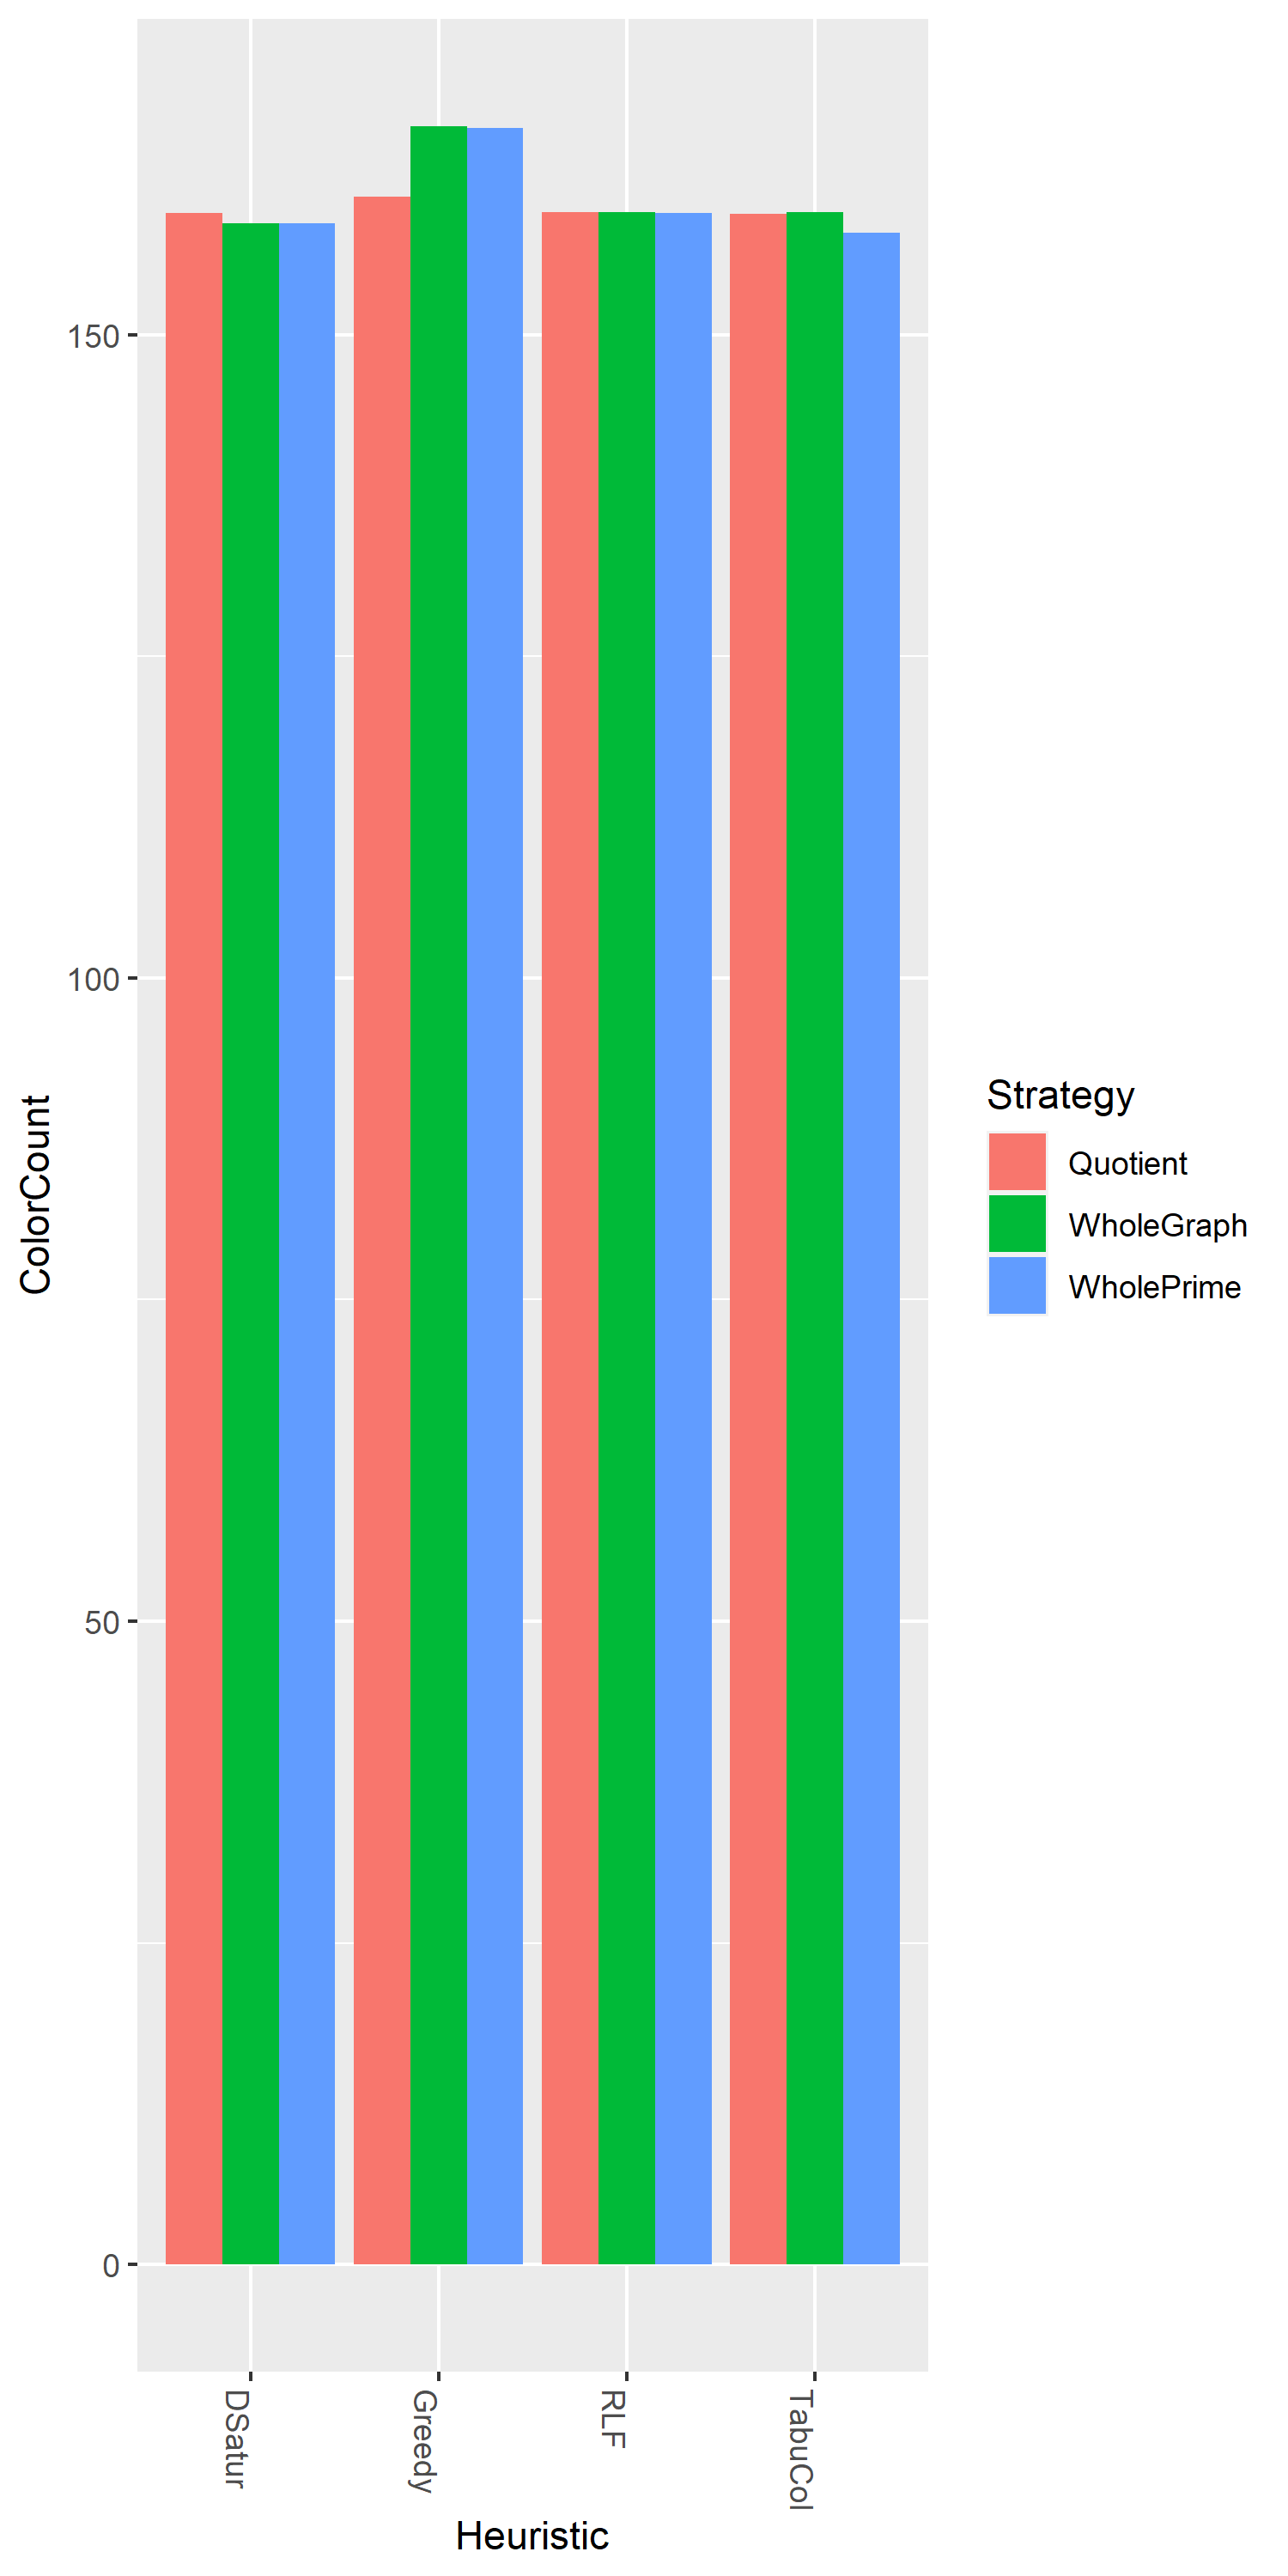
\includegraphics[width=\columnwidth]{Tables/Generated.png}
      \caption{Coloring results}
      \label{fig:generatedc}
    \end{subfigure}%
    \begin{subfigure}{.4\paperwidth}
        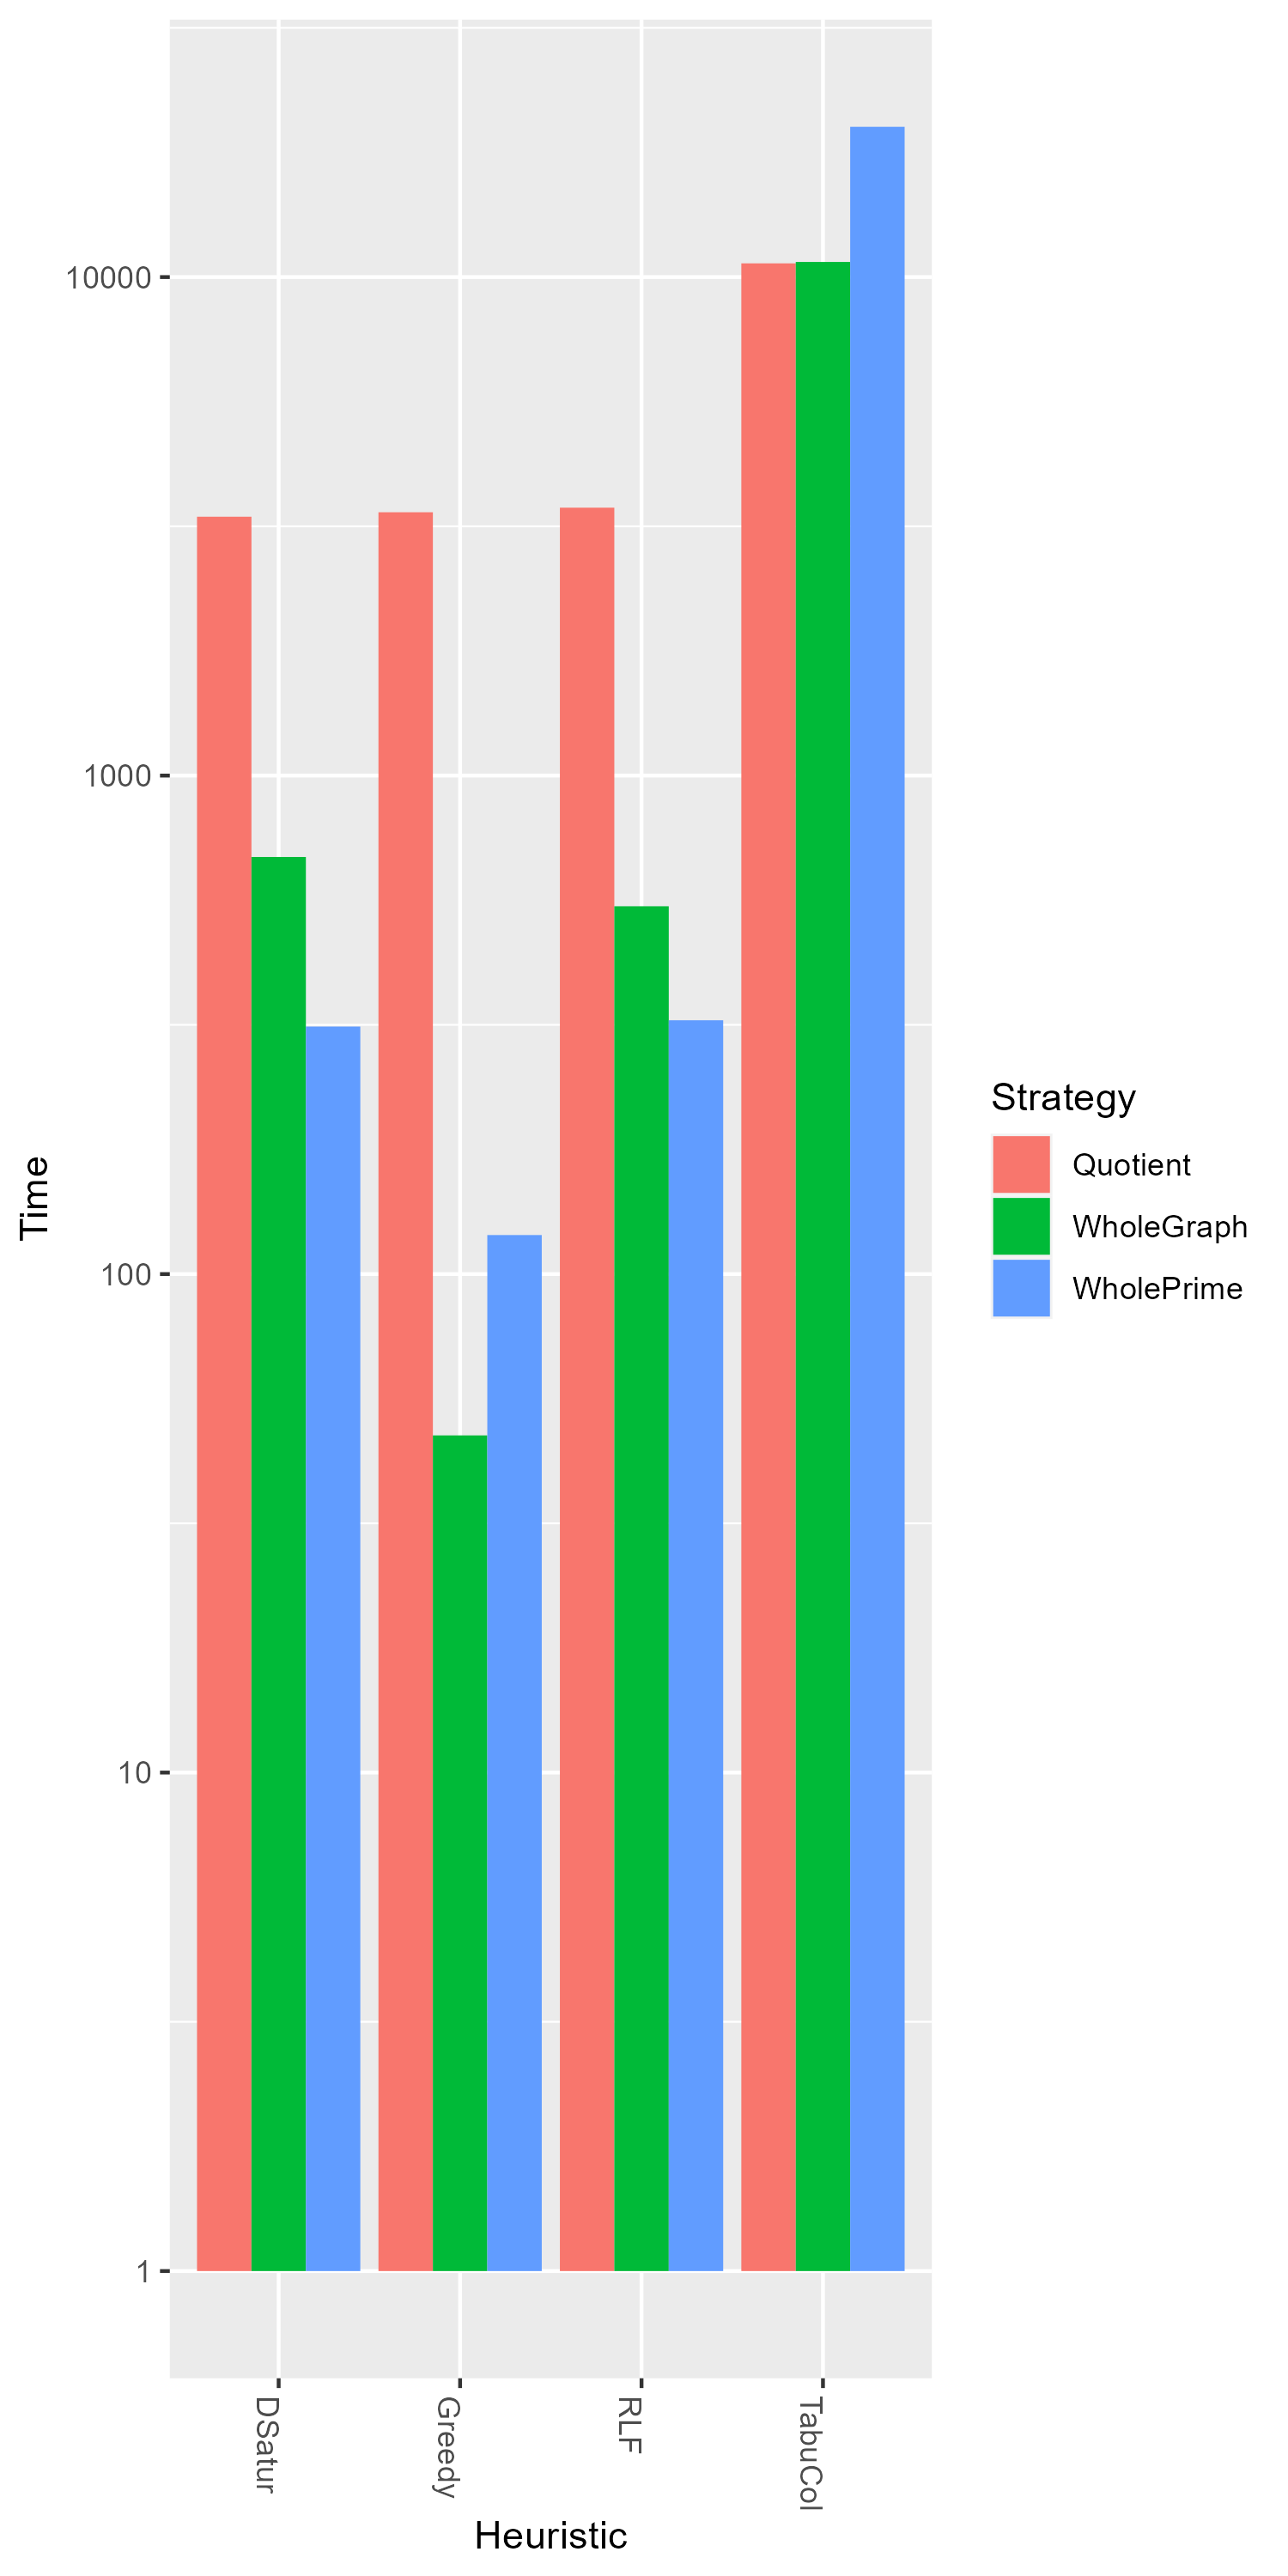
\includegraphics[width=\columnwidth]{Tables/GeneratedTime.png}
      \caption{Runtime}
      \label{fig:generatedt}
    \end{subfigure}
\caption{Combined results for all generated graphs. \figdesc}
\label{fig:generated}
\end{figure}

\FloatBarrier
\subsection{Discussion}

Something that we can see from the tables, most easily from
\autoref{fig:generated}, is that applying a heuristic locally on prime modules
doesn't significantly affect the resulting color for RLF,Greedy and Dsatur. It
does however seem to give a minor improvement for TabuCol. In situations where
one would consider using TabuCol with it's comparably larger execution time in
the first place, so could it be reasonable to use the modular decomposition for
increased performance.

Looking at the difference between series probability of 35\% versus 70\%, it
seems like the performance for TabuCol is better for the sparser graph with
35\% series probability. There also doesn't seem to be any direct difference
with the number of prime modules, both 10 and 5 seem to perform similarly.

The result for the quotient strategy always seems comparable to the performance
of RLF. It can be seen to outperform pure RLF very slightly for some
combinations, such as in \autoref{fig:dimacs}. It also exhibits a much larger
runtime, most notable for the same DIMACS test set in \autoref{fig:dimacs}.  The
potential performance benefit most likely doesn't compensate for the increased
runtime however, even with a more optimized implementation.

Looking at the time taken to color the graphs, we can see that the modular
decomposition might have a use in decreasing the execution time. Graph coloring
algorithms with execution time that doesn't scale linearly with the size of the
graph could benefit from being applied more times on smaller subgraphs. But
whether or not this is worth it in practice depends on the ability to implement
the modular decomposition tree in linear time, and if the added computations
can be compensated by large enough graphs.

Another possible advantage with the modular decomposition is that it could
allow for more easily implemented parallelised coloring algorithms. As the
child modules of a module in the modular decomposition tree creates a partition
of the parent module, so can the different parts of the modular decomposition
tree be colored in parallel, which could compensate for the increased runtime
when for example using TabuCol.

\section{Conclusion}

Using the modular decomposition didn't significantly improve the performance of
the tested algorithms, except in the case for TabuCol. This does show that
performance benefit can vary from algorithm to algorithm, but the total
difference is also most likely relatively small. The modular decomposition
coloring does however show some potential in improving the runtime for
different coloring algorithms, and combined with parallelised coloring of prime
modules might lead to larger improvements when examining colors relative to
time taken.

The coloring was mostly improved when using TabuCol, and it's possible that
other similar algorithms could see an improvement as well. It's also possible
that there are other ways to utilise the modular decomposition when coloring
prime modules other than the quotient strategy. 

Another area worth investigating is finding examples of real-world graphs that
have modular decomposition without a prime root module. The  parameters set for
the generated graphs might be different from graphs encountered in real-world
use cases, and could exhibit different properties that make them more/less
suitable for these coloring methods.



\printbibliography

\newpage
\Baksida %Kommentera för att bli av med loggan
\vspace*{13cm}
%Kandidatuppsats 2010:11\\ %Fyll i löpnummer
Datalogi\\
%September 2010\\\\ % Fyll i månad och år
\monthyeardate\today\\
www.math.su.se\\\\
Beräkningsmatematik\\
Matematiska institutionen\\
Stockholms universitet\\
106 91 Stockholm\\

\end{document}
